% ==========================================
% Curated book edition: XHIGH (300k 1-part Long Decode) base integrated into book
% Preserves Week 7 Tuesday / Week 8 cross-references & theorem/proposition labels,
% adds \recap links, and retains all updated TikZ figures, speech, and board notes.
% ==========================================
% ==========================================
% Step 4/4 - Final refinement (refinement step 3)
% Output: step4-10-28-2026-wednesday-week7-Algebra_I-final.tex
% Input: step3-10-28-2026-wednesday-week7-Algebra_I-speech_refined.tex
% Model: gemini-4-hydrogen
% Temperature: 0.35
% TopP: 0.9
% TopK: 10
% MaxOutputTokens: 300000
% ThinkingBudget: 4096
% ThinkingLevel: XHIGH
% Processed on: 2026-11-14 10:58:08
% Thought summaries: step4-10-28-2026-wednesday-week7-Algebra_I-final-thoughts.md
% ------------------------------------------
% Token Usage (2 Request(s)):
%   - Total Prompt Tokens : 199'159 (gesamter Prompt, inkl. Cache)
%   - Cached Context      : 0 (aus Google Context-Cache, rabattiert)
%   - Fresh Input Tokens  : 199'159 (neu verrechneter Input)
%   - Output Tokens       : 34'231 (generiertes LaTeX, ohne Thinking)
%   - Thinking Tokens     : 59'393 (Denk-Tokens, als Output verrechnet)
% ==========================================
% ==========================================
% Step 3/4 - Speech refinement (refinement step 2)
% Output: step3-10-28-2026-wednesday-week7-Algebra_I-speech_refined.tex
% Input: step1-10-28-2026-wednesday-week7-Algebra_I.tex
% Model: gemini-4-hydrogen
% Temperature: 0.35
% TopP: 0.9
% TopK: 10
% MaxOutputTokens: 300000
% ThinkingBudget: 4096
% ThinkingLevel: XHIGH
% Processed on: 2026-11-14 10:41:52
% Thought summaries: step3-10-28-2026-wednesday-week7-Algebra_I-speech_refined-thoughts.md
% Non-speech guard: not applied (speech begin/end tags do not alternate in the input, line 942); the answer is used unchecked outside speech
% ------------------------------------------
% Token Usage (2 Request(s)):
%   - Total Prompt Tokens : 424'067 (gesamter Prompt, inkl. Cache)
%   - Cached Context      : 0 (aus Google Context-Cache, rabattiert)
%   - Fresh Input Tokens  : 424'067 (neu verrechneter Input)
%   - Output Tokens       : 33'039 (generiertes LaTeX, ohne Thinking)
%   - Thinking Tokens     : 77'611 (Denk-Tokens, als Output verrechnet)
% ==========================================
% ==========================================
% Step 1/4 - Transcription (single part, 1 of 1)
% Output: step1-10-28-2026-wednesday-week7-Algebra_I.tex
% Source video: 10-28-2026-wednesday-week7-Algebra_I-speed-1-compressed.mp4
% Source segment: 10-28-2026-wednesday-week7-Algebra_I.mp4
% Model: gemini-4-hydrogen
% Temperature: 0.36
% TopP: 0.95
% TopK: 40
% MaxOutputTokens: 300000
% ThinkingBudget: 32765
% ThinkingLevel: XHIGH
% Processed on: 2026-11-14 10:28:56
% Thought summaries: step1-10-28-2026-wednesday-week7-Algebra_I-thoughts.md
% ------------------------------------------
% Token Usage (2 Request(s)):
%   - Total Prompt Tokens : 1'223'002 (gesamter Prompt, inkl. Cache)
%   - Cached Context      : 0 (aus Google Context-Cache, rabattiert)
%   - Fresh Input Tokens  : 1'223'002 (neu verrechneter Input)
%   - Output Tokens       : 33'700 (generiertes LaTeX, ohne Thinking)
%   - Thinking Tokens     : 72'542 (Denk-Tokens, als Output verrechnet)
% ==========================================

% Primary Language: English
% End of the video: 00:43:54
% Lecturer(s): Unknown

\lecturechapter[7]{Wednesday}{28 Oct}{28 October 2026}{Lagrange's Theorem, Symmetric Groups, and Symmetries of Platonic Solids}

\begin{overview}[Context and Overview]
This lecture continues the study of groups with a focus on finite and non-Abelian groups, moving from element orders to Lagrange's theorem and concrete geometric examples of finite symmetry groups:
\begin{itemize}
    \item \textbf{Review of Groups and Cyclic Subgroups:} Contrasting symmetric groups $S_n$ and cyclic Abelian groups $\faktor{\mathbb{Z}}{n\mathbb{Z}}$; reviewing element order $\operatorname{Ord}(x)$ and proving that $\langle x \rangle \subset G$ is a subgroup isomorphic to $(\faktor{\mathbb{Z}}{\operatorname{Ord}(x)\mathbb{Z}}, +, 0)$.
    \item \textbf{Lagrange's Theorem:} Motivating divisibility of $|G|$ via element orders in $S_3$, stating Lagrange's theorem ($|H| \mid |G|$ for any subgroup $H \subset G$ of a finite group $G$), and proving it using an equivalence relation on $G$ and a bijection $\phi \colon H \to E$ onto each equivalence class.
    \item \textbf{Cycle Decomposition in $S_n$:} Visualizing permutations $\sigma \in S_7$ dynamically on $[7]$ to obtain disjoint cycle decompositions and integer partitions.
    \item \textbf{Symmetries of the Platonic Solids:} Counting rotational symmetries of the cube ($24$), tetrahedron ($12$), and octahedron ($24$), formulating the geometric isomorphism $\operatorname{Rot}(\text{Cube}) \cong S_4$ via the four long diagonals, and identifying $\operatorname{Rot}(\text{Tetrahedron}) \cong A_4$ inside $S_4$.
\end{itemize}
\end{overview}

\section{Review of Groups and Cyclic Subgroups}

\subsection{Finite and Non-Abelian Groups}

\begin{speech}[00:00:00 - 00:01:02]
Okay, so, we start. I hope you have now concluded your study of Confucius, Plato, and Schopenhauer, and we can come back to the discussion of groups.

So, I defined last time group, $G$ is a group, which I don't repeat now \inlinemetanote{writes \qt{$G$ group} and \qt{$(G, \cdot, e)$}}. And I remind you --- because it's kind of important for the perspective of the discussion about group theory --- that we will normally... or our interest will be here mainly, but not exclusively, focused on finite groups, but not always \inlinemetanote{writes: $\Rightarrow$ Mainly focused on finite grps.}.

And also our main interest, but not always, is on non-commutative groups \inlinemetanote{writes: $\Rightarrow$ on non-Abelian.}. So, non-Abelian. But not always. So, you should have in your mind: when I say \qt{group}, it's a finite group, and not necessarily Abelian.
\end{speech}

\begin{content}[Scope and Perspective of the Group Theory Discussion]
\recap{Groups $(G, \cdot, e)$ were defined in the previous lecture (\cref{def:group-w7tue}).}

Let $(G, \cdot, e)$ denote a group with group operation $\cdot$ and neutral element $e$ (as defined in the previous lecture). Throughout our study of group theory, our primary focus will be on:
\begin{itemize}
    \item \textbf{Finite Groups:} Groups $G$ with finitely many elements ($|G| < \infty$), though infinite groups are not excluded.
    \item \textbf{Non-Abelian Groups:} Groups in which the operation $\cdot$ is not necessarily commutative ($xy \neq yx$ in general).
\end{itemize}
\end{content}

\begin{speech}[00:01:02 - 00:02:02]
So, the two examples, the two families of examples on extremes, are the family of the symmetric groups $S_n$ \inlinemetanote{writes: $S_n$} --- we'll say more, I said a little bit about this before, but I will say more --- symmetric group, and this is of course a finite group of size $n$ factorial \inlinemetanote{writes \qt{Symmetric grp} and \qt{$|S_n| = n!$}}. And that's somehow the richest family that we will speak about, and in some sense --- in a sense I'll make precise later --- really a very rich family of finite groups, maybe the richest family of finite groups.

And then there's the simplest family, $\mathbb{Z} \bmod n\mathbb{Z}$, that's with $+$ and $0$ \inlinemetanote{writes: $(\faktor{\mathbb{Z}}{n\mathbb{Z}}, +, 0)$}. These are the Abelian groups we've seen before, and these are called cyclic. So, this is the word we haven't really used before: \newterm{cyclic} Abelian \inlinemetanote{writes: cyclic abelian}. If you meet someone and they say they're considering a cyclic Abelian group of order $n$, they mean this group, exactly this group. It's cyclic --- well, it's because the one element generates it all in a big cycle.
\end{speech}

\begin{content}
\begin{examples}[Extreme Families of Finite Groups]
\label[examples]{exm:extreme-families-groups}
We contrast two fundamental families at opposite extremes of complexity:
\begin{enumerate}[label=\textbf{\arabic*.}]
    \item \textbf{The Symmetric Groups $S_n$:} The symmetric group on $n$ elements (\cref{def:symmetric-group}) is a finite (in general non-Abelian for $n \ge 3$, \cref{obs:s3-non-commutative}) group of order (\cref{prop:order-symmetric-group}):
    \[
    |S_n| = n!
    \]
    It represents the richest family of finite groups we will study.
    \item \textbf{Cyclic Abelian Groups $\faktor{\mathbb{Z}}{n\mathbb{Z}}$:} The additive group of integers modulo $n$,
    \[
    \left(\faktor{\mathbb{Z}}{n\mathbb{Z}}, +, 0\right),
    \]
    is the simplest family of finite groups. Such a group is called \newterm{cyclic} (and Abelian) because a single element (such as the residue class $\bar{1}$, \cref{def:residue-class-ring}) generates the entire group in one cycle.
\end{enumerate}
\end{examples}
\end{content}

\subsection{Order of an Element and Subgroup Generated by an Element}

\begin{speech}[00:02:02 - 00:03:18]
So, we were discussing in the second period last time: the setup of the discussion was $G$ is a group, and a finite one, and $x$ is an element \inlinemetanote{draws a double vertical line divider and writes \qt{$G$ is group,}, \qt{finite}, and \qt{$x \in G$}}.

And we had proven some things already. So, we had defined --- it's kind of a theorem-definition --- we had seen that the order of $x$ is well-defined \inlinemetanote{writes \qt{\textbf{(1)} We had seen the} and \qt{order of $x$ is well-defined.}}.

And I'll just remind you what the order is: this order of $x$ is the minimal $m$, a positive integer, such that $x$ to the $m$ is the neutral element in $G$ \inlinemetanote{writes \qt{$\operatorname{Ord}(x) =$} and \qt{the min $m > 0$ s.t. $x^m = e \in G$}}. So, to say it's well-defined, you have to first show that there exists some, and then it's a non-empty set and you can pick the minimal one. So, we proved all of this last time.
\end{speech}

\begin{content}[Recap: Order of an Element in a Finite Group]
\recap{The order of an element was defined in the previous lecture (\cref{def:element-order}), which showed that it is well-defined (\cref{prop:finite-group-identity-power}).}

Let $G$ be a finite group and let $x \in G$.

\begin{definition}[Order of an Element]\label[definition]{def:order-of-element}
\textbf{(1)} As established previously, the \newterm{order} of $x$, denoted $\operatorname{Ord}(x)$, is well-defined and given by the minimal positive integer $m > 0$ such that $x^m = e \in G$:
\[
\operatorname{Ord}(x) := \min \{ m \in \mathbb{Z}_{>0} \mid x^m = e \}.
\]
\end{definition}

\begin{steps}[Why Well-Definedness Requires Proof]
To establish that $\operatorname{Ord}(x)$ is well-defined for a finite group $G$, one first shows (by the pigeonhole principle applied to the powers $e, x, x^2, \dots$ together with group cancellation, \cref{prop:cancellation-laws}) that the set $\{ m > 0 \mid x^m = e \}$ is non-empty (\cref{prop:finite-group-identity-power}). The Well-Ordering Principle on $\mathbb{Z}_{>0}$ (\cref{fact:pre-well-ordering}) then guarantees the existence of a unique minimal element.
\end{steps}
\end{content}

\begin{speech}[00:03:18 - 00:04:05]
And I think that the point where I stopped was this discussion: so, another definition is I use these triangular parentheses, the triangle brackets \inlinemetanote{writes: (ii) $\langle x \rangle$}. This is by definition the set of elements that includes the neutral element, $x$, $x^2$, all the way to $x$ to the order of $x$ minus $1$ \inlinemetanote{writes \qt{$\stackrel{\text{def}}{=} \langle e, x, x^2, \dots, x^{\operatorname{Ord}(x)-1} \rangle \subset G$}, using angle brackets on the right as a slip for set braces}. Okay, this is a subset of $G$. That's a definition; sometimes in words this is the... well, let me say the words later. So, that's where we were last time. Are there questions about this? That's in my memory where we were last time.
\end{speech}

\begin{content}
\recap{This is \cref{def:cyclic-subgroup} of the previous lecture, where \cref{lem:cyclic-subgroup-order} showed that the listed powers are distinct. That $\langle x \rangle$ is a subgroup isomorphic to $(\faktor{\mathbb{Z}}{\operatorname{Ord}(x)\mathbb{Z}}, +, 0)$ was stated there (\cref{prop:cyclic-isomorphism}) and is proved next.}

\begin{definition}[Powers Generated by \texorpdfstring{$x$}{x}]\label[definition]{def:powers-subset}
\textbf{(2)} For an element $x \in G$ of a finite group $G$, we define the subset $\langle x \rangle \subset G$ by:
\[
\langle x \rangle \stackrel{\text{def}}{=} \{ e, x, x^2, \dots, x^{\operatorname{Ord}(x)-1} \} \subset G.
\]
\end{definition}
\end{content}

\begin{aiNote}[Board Notation Conventions: \texorpdfstring{$\subset$}{subset} and Angle-Bracket Slip]
% [PERSISTENT]
Two conventions from the blackboard are noted here:
\begin{itemize}
    \item As everywhere in these notes (\cref{not:subset-board}), $\subset$ stands for any subset or subgroup, proper or not; many textbooks write $\subseteq$ or $\le$.
    \item In defining $\langle x \rangle$ on the board, the lecturer wrote $\langle x \rangle \stackrel{\text{def}}{=} \langle e, x, x^2, \dots, x^{\operatorname{Ord}(x)-1} \rangle \subset G$, repeating the angle brackets $\langle \dots \rangle$ on the right-hand side as a slip for set braces $\{ \dots \}$. In the formal definition above, standard set braces are used.
\end{itemize}
\end{aiNote}

\begin{speech}[00:04:05 - 00:04:19]
So, the statement now, proposition, is that this subset in $G$ is a subgroup \inlinemetanote{writes: Prop. $\langle x \rangle \subset G$ is a subgroup.}.
\end{speech}

\begin{content}
\begin{proposition}\label[proposition]{prop:cyclic-subgroup}
Let $G$ be a finite group and $x \in G$. Then $\langle x \rangle \subset G$ is a subgroup of $G$.
\end{proposition}
\end{content}

\begin{proofWrapper}[Proof of \cref{prop:cyclic-subgroup}]
\begin{speech}[00:04:19 - 00:05:34]
All right, and what's the proof \inlinemetanote{writes: Proof:}? Well, to check it's a subgroup, I have to check several things. The first is that this subset is closed under the group product \inlinemetanote{writes: $\langle x \rangle$ is closed under $\cdot$}. Okay? So, I have to check that.

So, is this true? That means I take some person here, $x^k$, and take another one, $x^\ell$, and I apply the group product; this is $x$ $k$ times, this is $x$ $\ell$ times, so when I put them together, I get $x$ $k+\ell$ times \inlinemetanote{writes \qt{$x^k \cdot x^\ell$} and \qt{$= x^{k+\ell}$}, and indicates $k$ and $\ell$ factors of $x$ underneath}.

And then I get slightly worried because $k + \ell$ might be bigger than this \inlinemetanote{points at $\operatorname{Ord}(x)-1$}, but of course, we know that $x$ to the $\operatorname{Ord}$ is $e$, is the neutral element, so I can keep removing this; so, all that matters is that it's the residue modulo this number \inlinemetanote{writes \qt{$x^{\operatorname{Ord}(x)} = e$} and writes \qt{$\bmod \operatorname{Ord}$} above $k + \ell$}. Is that clear? So, I hope that's clear: it's closed under product, because if I come up over here, I can always take out the $\operatorname{Ord}(x)$ part, because it's just the neutral element.
\end{speech}

\begin{content}[Closure Under the Group Product]
We verify the three subgroup criteria for $\langle x \rangle \subset G$.

\textbf{Closure under $\cdot$:} Let $x^k, x^\ell \in \langle x \rangle$, where $0 \le k, \ell \le \operatorname{Ord}(x) - 1$. Multiplying them gives:
\[
x^k \cdot x^\ell = \underbrace{(x \cdots x)}_{k \text{ times}} \cdot \underbrace{(x \cdots x)}_{\ell \text{ times}} = x^{k+\ell}.
\]
Even if $k + \ell \ge \operatorname{Ord}(x)$, we know that $x^{\operatorname{Ord}(x)} = e$, so factors of $x^{\operatorname{Ord}(x)}$ can be repeatedly removed without changing the element. Only the remainder of $k + \ell$ modulo $\operatorname{Ord}(x)$ matters.

\begin{steps}[Formalizing the Reduction via Division with Remainder]
By Euclidean division, write $k + \ell = q \cdot \operatorname{Ord}(x) + r$ for some integer $q \ge 0$ and remainder $0 \le r \le \operatorname{Ord}(x) - 1$. Then:
\[
x^{k+\ell} = x^{q \cdot \operatorname{Ord}(x) + r} = \left(x^{\operatorname{Ord}(x)}\right)^q \cdot x^r = e^q \cdot x^r = x^r \in \langle x \rangle.
\]
Hence, $\langle x \rangle$ is closed under the group product.
\end{steps}
\end{content}

\begin{speech}[00:05:34 - 00:06:34]
Okay, so, then we have to show that... well, I should have said this first: $e$ is in here, but that was just in the list \inlinemetanote{writes: $e \in \langle x \rangle \ \checkmark$}.

And the last one we have to show is that if someone is here, then the inverse is also here \inlinemetanote{writes: if $y \in \langle x \rangle$, then $y^{-1} \in \langle x \rangle$}. So, this should also be clear: if I pick one of these elements $x^k$, where $k$ is in this list, I can always multiply it by $x$ to the $\operatorname{Ord}(x) - k$, and it will also be in this list, unless $k$ is $0$ \inlinemetanote{writes: $x^{\operatorname{Ord}(x)-k}$} --- there's a boundary case you can check, but it's fine also.

But this times this is equal to $x$ to the $\operatorname{Ord}(x)$, which is $e$ \inlinemetanote{writes: $x^k \cdot x^{\operatorname{Ord}(x)-k} = x^{\operatorname{Ord}(x)} = e$}. So, that means the inverse is also in this list. Okay? So, all these three things are satisfied, and it is a fact that this construction --- if I take $x$ and I take the neutral element and I go all the way up to the order minus $1$ --- is a nice subset and it is a subgroup.
\end{speech}

\begin{content}[Neutral Element and Closure Under Inverses]
\textbf{Neutral element:} Directly from the definition of $\langle x \rangle$, we have $e \in \langle x \rangle$.

\textbf{Closure under inverses:} Let $y \in \langle x \rangle$, so $y = x^k$ for some $0 \le k \le \operatorname{Ord}(x) - 1$.
\begin{itemize}
    \item If $k = 0$, then $y = x^0 = e$, whose inverse is $e^{-1} = e \in \langle x \rangle$.
    \item If $1 \le k \le \operatorname{Ord}(x) - 1$, then $1 \le \operatorname{Ord}(x) - k \le \operatorname{Ord}(x) - 1$, so $x^{\operatorname{Ord}(x)-k} \in \langle x \rangle$. Multiplying gives:
    \[
    x^k \cdot x^{\operatorname{Ord}(x)-k} = x^{\operatorname{Ord}(x)} = e,
    \]
    and symmetrically $x^{\operatorname{Ord}(x)-k} \cdot x^k = x^{\operatorname{Ord}(x)} = e$. Thus, $y^{-1} = x^{\operatorname{Ord}(x)-k} \in \langle x \rangle$.
\end{itemize}
All three subgroup conditions hold, so $\langle x \rangle \subset G$ is a subgroup.
\end{content}
\end{proofWrapper}

\begin{speech}[00:06:34 - 00:07:24]
And moreover, if you understood what this product rule is, where you take this and this --- and maybe I'll just write it is equal to $r$, where $r$ is $k + \ell \bmod$ the order \inlinemetanote{writes \qt{$= x^r$} and \qt{$r = k+\ell \bmod \operatorname{Ord}$}} --- if you understand this product rule, I write it as a corollary, maybe it's a corollary of the proof: actually, this group is isomorphic to $\mathbb{Z} \bmod \operatorname{Ord}(x)\mathbb{Z}$ with addition and $0$ \inlinemetanote{writes: Cor: $\langle x \rangle \cong (\faktor{\mathbb{Z}}{\operatorname{Ord}(x)\mathbb{Z}}, +, 0)$}. Okay?
\end{speech}

\begin{content}[Structure of \texorpdfstring{$\langle x \rangle$}{<x>}]
From the proof above, for any integers $k, \ell \ge 0$ (in particular, $0 \le k, \ell < \operatorname{Ord}(x)$), the product of powers satisfies:
\[
x^k \cdot x^\ell = x^{k+\ell} = x^r, \qquad \text{where } r = (k + \ell) \bmod \operatorname{Ord}(x).
\]

\begin{corollary}\label[corollary]{cor:cyclic-subgroup-isomorphism}
For any element $x$ of a finite group $G$, there is a group isomorphism:
\[
\langle x \rangle \cong \left(\faktor{\mathbb{Z}}{\operatorname{Ord}(x)\mathbb{Z}}, +, 0\right).
\]
\end{corollary}

\begin{steps}[Explicit Isomorphism and Distinctness of Powers]
The map $\psi \colon \faktor{\mathbb{Z}}{\operatorname{Ord}(x)\mathbb{Z}} \to \langle x \rangle$ sending $\bar{k} \mapsto x^{k \bmod \operatorname{Ord}(x)}$ (or simply $\bar{k} \mapsto x^k$ for $0 \le k < \operatorname{Ord}(x)$) is well-defined and a homomorphism precisely because $x^k \cdot x^\ell = x^r$ with $r = (k+\ell) \bmod \operatorname{Ord}(x)$. Moreover, the elements $e, x, x^2, \dots, x^{\operatorname{Ord}(x)-1}$ are pairwise distinct (\cref{lem:cyclic-subgroup-order}): if $x^i = x^j$ for $0 \le i < j < \operatorname{Ord}(x)$, then $x^{j-i} = e$ with $0 < j - i < \operatorname{Ord}(x)$, contradicting the minimality of $\operatorname{Ord}(x)$. Hence, $|\langle x \rangle| = \operatorname{Ord}(x)$ and $\psi$ is a bijection.
\end{steps}
\end{content}

\begin{speech}[00:07:24 - 00:07:55]
And the words for this --- now I tell you the words because I didn't want to bias the issue --- is that this symbol... the words for it is the \newterm{subgroup generated by} the element $x$ \inlinemetanote{writes: $\langle x \rangle \subset G$, \qt{Subgroup gen. by $x$}}. Okay? I didn't want to say at the beginning because then it'd bias the issue, but now we know it's a subgroup, I can say.
\end{speech}

\begin{content}
\begin{definition}[Subgroup Generated by an Element]\label[definition]{def:subgroup-generated}
Given a finite group $G$ and $x \in G$, the subgroup $\langle x \rangle \subset G$ is called the \newterm{subgroup generated by $x$}.
\end{definition}
\end{content}

\begin{hidden}
% timestamp: 00:07:55
% topic: Review of element order, cyclic subgroup <x>, and isomorphism with Z/ord(x)Z
% board_state: def:order-of-element, def:powers-subset, prop:cyclic-subgroup, cor:cyclic-subgroup-isomorphism, def:subgroup-generated
% next_goal: Motivate Lagrange's theorem using element orders in S_3, state and prove Lagrange's theorem.
% open_loops: none
\end{hidden}

\section{Lagrange's Theorem}

\subsection{Motivation: Element Orders in \texorpdfstring{$S_3$}{S3} and Statement of Lagrange's Theorem}

\begin{speech}[00:07:55 - 00:08:57]
All right, so, like in our example for $S_3$, we had some elements like these $2$-cycles, this element --- and I said sometimes I write this, sometimes I don't; it's just, you know, however I feel --- but often people don't write the singletons \inlinemetanote{writes: $S_3$, $(1\,2)(3)$}.

If I take this element, we saw it has order $2$, so this has order $2$, and this has order $3$ \inlinemetanote{writes \qt{$\rightsquigarrow \operatorname{Ord} = 2$} and \qt{$(1\,2\,3) \rightsquigarrow \operatorname{Ord} = 3$}}.

And one of the things you notice here is: what is the order of this group? It's $3$ factorial, which is $6$ \inlinemetanote{writes: $|S_3| = 3! = 6$}. So, we find here the orders of the elements --- at least in this example --- orders of elements seem to divide the order of the group, at least in this case \inlinemetanote{writes: $\operatorname{Ord}\text{s of elmts.} \mid |S_3|$}. So, you can wonder whether this is always the case. So, this is a kind of interesting question.
\end{speech}

\begin{content}
\begin{example}[Orders of Elements in \texorpdfstring{$S_3$}{S3}]
\label[example]{ex:s3-element-orders}
Consider the symmetric group $S_3$ (\cref{ex:orders-s3}), which has order $|S_3| = 3! = 6$. Examining the orders of its elements (noting that $1$-cycles such as $(3)$ are often omitted in cycle notation, \cref{def:cycle}):
\begin{align*}
(1\,2)(3) &\rightsquigarrow \operatorname{Ord} = 2, \\
(1\,2\,3) &\rightsquigarrow \operatorname{Ord} = 3.
\end{align*}
In this group, both $2$ and $3$ divide $6$:
\[
\text{Orders of elements} \mid |S_3|.
\]
\end{example}
\end{content}

\begin{speech}[00:08:57 - 00:10:04]
So, I said, like, this kind of question is a question about finite groups. Because if $G$ has infinite order, we can't really talk... well, if $G$ was a group with infinite order, the elements may not have finite order, and in any case we can't talk about this division property. That's why I say we're focusing on finite groups.

So, anyway, in this case we find that the order of the elements divides the order of the group, so one can wonder: is this always the case \inlinemetanote{writes: Is this always true?}? So, specifically, if $x$ is an element of $G$, a finite group, does the order of $x$ divide the order of $G$ \inlinemetanote{writes: If $x \in G$ finite group, does $\operatorname{Ord}(x) \mid |G|$?}? That's a very specific question, and the answer is going to be yes \inlinemetanote{writes: YES}. And actually, the proof is that a much more general property holds, and that's the main topic of today's lecture...
\end{speech}

\begin{content}[Divisibility of Group Order by Element Order]
For an infinite group, elements need not have finite order, and divisibility of $|G|$ is not defined; thus, the divisibility question is specific to finite groups.

\begin{question}\label[question]{q:ord-divides-group}
If $G$ is a finite group and $x \in G$, does $\operatorname{Ord}(x) \mid |G|$ always hold?
\end{question}

\begin{answer}[to \cref{q:ord-divides-group}]\label[answer]{ans:ord-divides-group}
\textcolor{ForestGreen}{\textbf{Yes.}} This follows from a much more general theorem concerning all subgroups of a finite group.
\end{answer}
\end{content}

\begin{speech}[00:10:04 - 00:12:05]
...which is really, in some sense, usually the first theorem in finite group theory, and it's a theorem of Joseph-Louis Lagrange \inlinemetanote{writes: J. L. Lagrange}. And it's that if $H$ is a subgroup of $G$ \inlinemetanote{writes: If $H \subset G$} --- $H$ is a subgroup and $G$ is finite \inlinemetanote{writes: $H$ is subgroup and $G$ is finite} --- so that's the hypothesis: we have a finite group and a subgroup. I don't have to say the subgroup is finite because once the group is finite, the subgroup is also finite. So, then --- this is what Joseph-Louis says --- the order of $H$ always divides the order of $G$ \inlinemetanote{writes: Then: $|H| \mid |G|$}. Okay?

So, it's usually the very first actual theorem about finite groups, and I'll prove it --- the proof is simple, it's conceptual. One interesting thing is that he lived in the $18$th century, and the definition of a group came like half a century after he passed away, so you can wonder: how did he prove this theorem? And, you know, of course he didn't prove this theorem. He proved something about symmetric groups that people have interpreted to be this theorem \inlinemetanote{draws a double vertical line after the theorem}.

But this is the same Lagrange that's responsible for Lagrangian mechanics and the calculus of variations, which is a fantastic topic. Whether that's covered in the math curriculum, I don't know. Part of my life was a physicist, and I liked that part. That's a great topic. So, he's done a lot of amazing stuff. But you've taken this stuff like Lagrangian mechanics at some point? Calculus of variations, do you take that? Yeah. Those are really great subjects.
\end{speech}

\begin{content}
\begin{theorem}[Lagrange's Theorem]\label[theorem]{thm:lagrange}
Let $G$ be a finite group and let $H \subset G$ be a subgroup. Then the order of $H$ divides the order of $G$:
\[
|H| \mid |G|.
\]
\end{theorem}
\end{content}

\begin{insight}[Historical Context: Lagrange and the Origin of His Theorem]
Joseph-Louis Lagrange lived in the $18$th century, roughly half a century before the abstract definition of a group was formulated. Rather than proving \cref{thm:lagrange} for abstract finite groups, he proved a concrete result on symmetric groups that was later interpreted and generalized into the abstract theorem. He is also the same Lagrange celebrated for Lagrangian mechanics and the calculus of variations.
\end{insight}

\begin{aiNote}[Beyond the Lecture: Historical Origin of Lagrange's Theorem]
% [PERSISTENT, ADDITION]
Lagrange's original result on symmetric groups arose in his work on solving polynomial equations via permutations of their roots.
\end{aiNote}

\begin{speech}[00:12:05 - 00:12:34]
Okay, so, we're going to prove this \inlinemetanote{writes: Proof:}. So, is there any question about this theorem? And you see, this theorem certainly implies this \inlinemetanote{points at \cref{q:ord-divides-group}} statement, because if I have an element, the order of this element is the size of that subgroup \inlinemetanote{points at $\langle x \rangle$}. So, in particular, if every subgroup divides the order of $G$, the order always divides the order of $G$, okay?
\end{speech}

\begin{content}[Consequence for Element Orders]
\begin{corollary}[Element Order Divides Group Order]\label[corollary]{cor:ord-divides-group}
Let $G$ be a finite group and $x \in G$. Then $\operatorname{Ord}(x) \mid |G|$.
\end{corollary}

\begin{proof}
By \cref{prop:cyclic-subgroup}, $\langle x \rangle \subset G$ is a subgroup of $G$, and by \cref{cor:cyclic-subgroup-isomorphism} its order is $|\langle x \rangle| = \operatorname{Ord}(x)$. Applying Lagrange's theorem (\cref{thm:lagrange}) to $H = \langle x \rangle$ yields $\operatorname{Ord}(x) \mid |G|$.
\end{proof}
\end{content}

\begin{proofWrapper}[Proof of \cref{thm:lagrange}]
\subsection{Equivalence Relation on \texorpdfstring{$G$}{G} Induced by \texorpdfstring{$H$}{H}}

\begin{speech}[00:12:34 - 00:13:17]
So, then this is the much more general result. So, how are we going to prove it? It's an extremely nice proof, and... yeah. So, the proof is: we start by defining an equivalence relation on the set $G$ \inlinemetanote{writes: We start by defining an equivalence relation on set $G$.}. And then we will count $G$ by counting up the size of the equivalence classes. And this equivalence relation is just incredibly important for group theory, so we will define it.
\end{speech}

\begin{content}[Proof Strategy]
We start by defining a specific equivalence relation on the set $G$. Partitioning $G$ into its equivalence classes will allow us to count $|G|$ by summing the sizes of those equivalence classes.
\end{content}

\begin{speech}[00:13:17 - 00:14:52]
The notion of a group, while I erase I say, is that, you know, it has many fewer axioms than a ring, and in some sense it's a more primitive notion in mathematics, which means that it's more widely applicable and in some sense more fundamental than the notion of a ring \inlinemetanote{erases the upper-left and middle boards}. But the ring is motivated by number systems, so somehow it is a natural choice for the first topic in the course since most people have familiarity with number systems. But the group is a more ubiquitous notion because of course it has fewer axioms so you can find it more generally.

And it's motivated --- I mean, it has many motivations --- but a very strong motivation about the group is about symmetries of geometric objects. It's like a totally different motivation than a ring, which is about number systems that you encounter in school. So, while they're in the same class, and in some sense one thinks about them algebraically in the same space, the motivations that led to them are pretty much different, that I would say.

But they're both really amazingly interesting, intricate topics. And a lot of the moves, the algebraic moves, are similar; maybe that justifies having them in the same course. Sometimes the course is taught with groups first and then rings. I've taught it with rings first, then groups. It doesn't really matter, of course.
\end{speech}

\begin{insight}[Groups vs.\ Rings: Axiomatic Simplicity and Geometric Motivation]
Although groups and rings share similar algebraic techniques in the same course, they arise from very different motivations. Rings are modeled on familiar number systems, whereas groups have far fewer axioms and are strongly motivated by the symmetries of geometric objects --- making the group concept more primitive, fundamental, and ubiquitous across mathematics.
\end{insight}

\begin{speech}[00:14:52 - 00:15:48]
All right, so, for the proof of this theorem I'm going to define an equivalence relation. So, that means if you have $x$ and $y$ in $G$, I have to tell you how to define this relation \inlinemetanote{writes: $x, y \in G$}. The definition is that we say $x$ is related to $y$ if and only if --- it's a definition --- if there exists an $h$ in the subgroup such that $xh$ is equal to $y$ \inlinemetanote{writes: $x \sim y \stackrel{\text{def}}{\iff} \exists h \in H \text{ s.t. } xh = y$}. All right?

Now, you could say: why do I put $h$ on the right side? Could I put it on the left side? And you could do that. That would be your own equivalence relation, and it's totally equivalent for this proof and the proof will be fine, but since the groups are not commutative, not necessarily commutative, I have to decide, and I have decided to put it on the right, okay? That's the first comment.
\end{speech}

\begin{content}[Defining the Equivalence Relation on \texorpdfstring{$G$}{G}]
For elements $x, y \in G$, we define a binary relation $\sim$ on $G$ by:
\begin{equation}\label{eq:coset-equiv-relation}
x \sim y \stackrel{\text{def}}{\iff} \exists h \in H \text{ such that } xh = y.
\end{equation}

\begin{proposition}[Equivalence Relation Induced by a Subgroup]\label[proposition]{prop:equiv-relation-subgroup}
The relation $\sim$ defined in \eqref{eq:coset-equiv-relation} is an equivalence relation on $G$.
\end{proposition}

\begin{steps}[Choice of Right Multiplication]
Because $G$ is not necessarily commutative, multiplying by $h \in H$ on the right ($xh = y$) is in general different from multiplying on the left ($hx = y$). Defining the relation via $hx = y$ would produce a different equivalence relation, which would serve equally well for proving Lagrange's theorem; we simply fix the right-multiplication convention \eqref{eq:coset-equiv-relation}.
\end{steps}
\end{content}

\begin{aiNote}[Beyond the Lecture: Left and Right Cosets]
% [PERSISTENT, ADDITION]
The equivalence classes of the relation $x \sim y \iff \exists h \in H \colon xh = y$ are known in group theory as the \newterm{left cosets} $xH := \{xh \mid h \in H\}$ of $H$ in $G$. Using the alternative convention $hx = y$ yields the \newterm{right cosets} $Hx := \{hx \mid h \in H\}$ instead.
\end{aiNote}

\begin{speech}[00:15:48 - 00:16:15]
So, then for an equivalence relation, I have to check the properties. And normally I leave this to you, but here, this is so fundamental I'm going to do it --- it's probably a mistake, but nevertheless. So, the first property is that $x$ is related to itself \inlinemetanote{writes: $\bullet\ x \sim x$}. And that's if and only if I can find an $h$ in this group that satisfies that \inlinemetanote{points at $\exists h \in H \text{ s.t. } xh = y$}, and which one is that? Yeah?
\end{speech}

\begin{student}[Student Answer]
Neutral element.
\end{student}

\begin{speech}[00:16:17 - 00:17:27]
Neutral element. It's because $e$ has to be here because it's a subgroup, and then of course I have this equation, so that's fine \inlinemetanote{writes: $\iff e \in H, \ xe = x\;\checkmark$}.

Now, that's the reflexive... no, yeah, that's the reflexive property; then the symmetric property is: if $x$ is related to $y$, then $y$ is related to $x$ \inlinemetanote{writes: $\bullet\ x \sim y$ then $y \sim x$}. So, we have to prove this: $x$ is related to $y$ means that there exists an $h$ such that $xh = y$ \inlinemetanote{writes: $\iff xh = y$}. And then what do I write on the \qt{then} side \inlinemetanote{writes: then}?

If I have this, I can just multiply by $h^{-1}$, right? So, then I get... sorry... \inlinemetanote{wipes an aborted start and writes: $x = y h^{-1}$} so I can multiply by $h^{-1}$, which will make this $h$ go away and put an $h^{-1}$ there. And then this means that $y$ is related to $x$ --- I can write this again, if you really want to fit the definition \inlinemetanote{writes: $y h^{-1} = x$}. This says that $y$ is related to $x$, because if you have an element of $H$, the inverse is also in $H$. That's a property of being a subgroup. All right?
\end{speech}

\begin{content}[Verification of Reflexivity and Symmetry]
We verify the first two defining properties of an equivalence relation for $\sim$:

\textbf{Reflexivity ($x \sim x$):} For any $x \in G$, since $H \subset G$ is a subgroup, the neutral element satisfies $e \in H$, and
\[
x e = x \implies x \sim x.
\]

\textbf{Symmetry ($x \sim y \implies y \sim x$):} Suppose $x, y \in G$ satisfy $x \sim y$. By \eqref{eq:coset-equiv-relation}, there exists $h \in H$ such that $xh = y$. Multiplying both sides on the right by $h^{-1}$ gives:
\[
x = (xh)h^{-1} = y h^{-1} \implies y h^{-1} = x.
\]
Since $H$ is a subgroup and $h \in H$, we have $h^{-1} \in H$. Therefore, $y \sim x$.
\end{content}

\begin{speech}[00:17:27 - 00:18:54]
And the third one then is transitivity, which says that if I have $x$ related to $y$ and $y$ related to $z$, then I have to show that $x$ is related to $z$ \inlinemetanote{writes: $\bullet$ If $x \sim y$ and $y \sim z \implies x \sim z$}. And if I do this using the definition, this means that there exists some $h_1$ that satisfies this equation, and this one means there's some $h_2$ that satisfies this equation \inlinemetanote{writes \qt{$x h_1 = y$} and \qt{$y h_2 = z$}}. And then I have to find this relation equation \inlinemetanote{points at $x \sim z$}, and you can imagine what I do: I just take here $x h_1 h_2 = z$ \inlinemetanote{writes: $x h_1 h_2 = z$}. All right? And why does this work? It's because it's a subgroup, so $H$ is closed under product \inlinemetanote{writes: $H$ closed under $\cdot$}.

So, that's the proof that it's an equivalence relation, and you see the proof is perfect in a way that I need to check three properties to be an equivalence relation, and those are exactly the same three properties that $H$ is a subgroup. I've used everything exactly: the neutral element's there, it's closed under inverse, it's closed under product. So, in some sense, this statement that this definition is... on one hand, on this side it's an equivalence relation, and that side $H$ is a subgroup, they just perfectly align.
\end{speech}

\begin{content}[Verification of Transitivity]
\textbf{Transitivity (If $x \sim y$ and $y \sim z$, then $x \sim z$):} Suppose $x, y, z \in G$ satisfy $x \sim y$ and $y \sim z$. By definition \eqref{eq:coset-equiv-relation}, there exist elements $h_1, h_2 \in H$ such that
\[
x h_1 = y \qquad \text{and} \qquad y h_2 = z.
\]
Substituting $y = x h_1$ into the second equation and using associativity in $G$ yields:
\[
x (h_1 h_2) = (x h_1) h_2 = y h_2 = z.
\]
Since $H$ is a subgroup, $H$ is closed under the group product, so $h_1 h_2 \in H$. Hence, $x \sim z$.

Thus, $\sim$ is an equivalence relation on $G$, proving \cref{prop:equiv-relation-subgroup}.

\begin{steps}[Exact Alignment of Subgroup and Equivalence-Relation Axioms]
Notice how each equivalence-relation property corresponds one-to-one with a subgroup axiom of $H$:
\begin{itemize}
    \item \textbf{Reflexivity} $\longleftrightarrow$ $e \in H$ (existence of the neutral element).
    \item \textbf{Symmetry} $\longleftrightarrow$ $h \in H \implies h^{-1} \in H$ (closure under inverses).
    \item \textbf{Transitivity} $\longleftrightarrow$ $h_1, h_2 \in H \implies h_1 h_2 \in H$ (closure under the group product).
\end{itemize}
\end{steps}
\end{content}

\begin{hidden}
% timestamp: 00:18:54
% topic: Proof of Lagrange's Theorem: equivalence relation verified
% board_state: thm:lagrange, eq:coset-equiv-relation, prop:equiv-relation-subgroup
% next_goal: Partition G into equivalence classes, state |E_i| = |H|, construct bijection phi: H -> E
% open_loops: none
\end{hidden}

\subsection{Partition of \texorpdfstring{$G$}{G} into Equivalence Classes and the Claim \texorpdfstring{$|E_i| = |H|$}{|Ei| = |H|}}

\begin{speech}[00:18:54 - 00:20:32]
All right, so, we have proven that. Okay, so, now we have a picture: here is the group $G$, the finite group \inlinemetanote{draws a closed region labeled $G$}, so there's some people here \inlinemetanote{draws dots inside $G$}. And I have an equivalence relation, so whenever you have an equivalence relation, it divides the set into equivalence classes.

So, our equivalence relation divides it into equivalence classes: maybe here's one equivalence class, $E_1$ \inlinemetanote{draws a closed contour $E_1$ around two dots}, then there's some equivalence class here, $E_2$ \inlinemetanote{draws $E_2$ around three dots}, and then there's another equivalence class, $E_3$ \inlinemetanote{draws $E_3$ around two dots}. I don't know. There's finitely many --- it's a finite set, so there's finitely many equivalence classes --- so we can write an equation.

And this equation you can always write for equivalence classes on finite sets, and it's an equation that is so naive you think it couldn't possibly be useful. The equation is that the size of $G$ is equal to the sum from $i = 1$ to the $k$ --- which, $k$ is the number of equivalence classes \inlinemetanote{writes \qt{$|G| = \sum_{i=1}^k |E_i|$} and \qt{$k = \text{\# of equiv. classes}$}}. There's some finite number of equivalence classes, it's a finite group, you sum over the number of equivalence classes, and it's the size of the equivalence class.

So, that's the equation. It's a pretty naive equation; as I said, it looks so silly it seems hard to believe that it's useful, but it's just saying you take this $G$, equivalence relation, make some equivalence classes, and you account for everybody in $G$, and that equation just says you've accounted for everybody, exactly once.
\end{speech}

\begin{content}[Partition of \texorpdfstring{$G$}{G} into Equivalence Classes]
Because $\sim$ is an equivalence relation on the finite set $G$, it partitions $G$ into finitely many pairwise disjoint, non-empty equivalence classes $E_1, E_2, \dots, E_k$:

\definecolor{figBlue}{HTML}{076090} % RGB (7, 96, 144): petrol blue (MidnightBlue)
\definecolor{figGreen}{HTML}{3D8252} % RGB (61, 130, 82): dark green (ForestGreen!70!black)
\begin{hidden}
- Canvas: no scale, cm; G = ellipse centre (0, 0), radii 4.0 and 2.7; picture x in [-4.0, 4.4], y in [-2.7, 2.7]
- Order: (1) fill of G (figBlue!6); (2) fills of E_1, E_2, E_3 (figGreen!10); (3) outlines of G and E_1, E_2, E_3;
  (4) element dots inside each class; (5) all text last
- Containment check ((x/4.0)^2 + (y/2.7)^2 < 1):
  E_1: centre (-1.6, 0.95), radii 1.25 and 0.85 (x in [-2.85, -0.35], y in [0.10, 1.80]);
    farthest corner (-2.5, 1.55): (-2.5/4)^2 + (1.55/2.7)^2 = 0.39 + 0.33 = 0.72 < 1.
  E_2: centre (1.7, 0.15), radii 1.40 and 1.00 (x in [0.30, 3.10], y in [-0.85, 1.15]);
    farthest corner (2.7, 0.85): (2.7/4)^2 + (0.85/2.7)^2 = 0.46 + 0.10 = 0.56 < 1.
  E_3: centre (-1.1, -1.15), radii 1.25 and 0.80 (x in [-2.35, 0.15], y in [-1.95, -0.35]);
    farthest corner (-2.0, -1.75): (-2.0/4)^2 + (-1.75/2.7)^2 = 0.25 + 0.42 = 0.67 < 1.
- Disjointness: E_1 (x <= -0.35) vs E_2 (x >= 0.30): horizontal gap 0.65;
  E_1 (y >= 0.10) vs E_3 (y <= -0.35): vertical gap 0.45;
  E_2 (x >= 0.30) vs E_3 (x <= 0.15): horizontal gap 0.15, plus centres 1.3 apart in y.
- Dots: E_1 at (-2.1, 0.65), (-1.1, 0.65); E_2 at (1.1, -0.25), (1.7, -0.35), (2.3, -0.20);
  E_3 at (-1.6, -1.45), (-0.6, -1.45).
- Labels (normal size, 0.20 per character, height 0.45):
  "E_1" centred at (-1.6, 1.30): y in [1.08, 1.52], 0.28 below E_1 top (1.80), 0.43 above dots (0.65)
  "E_2" centred at (1.7, 0.55): y in [0.33, 0.77], 0.38 below E_2 top (1.15), 0.58 above dots (-0.20)
  "E_3" centred at (-1.1, -0.82): y in [-1.04, -0.60], 0.25 below E_3 top (-0.35), 0.41 above dots (-1.45)
  "G" anchor south west at (4.0 cos 35, 2.7 sin 35) = (3.28, 1.55), inner sep 0.15cm, outside G
\end{hidden}
\begin{center}
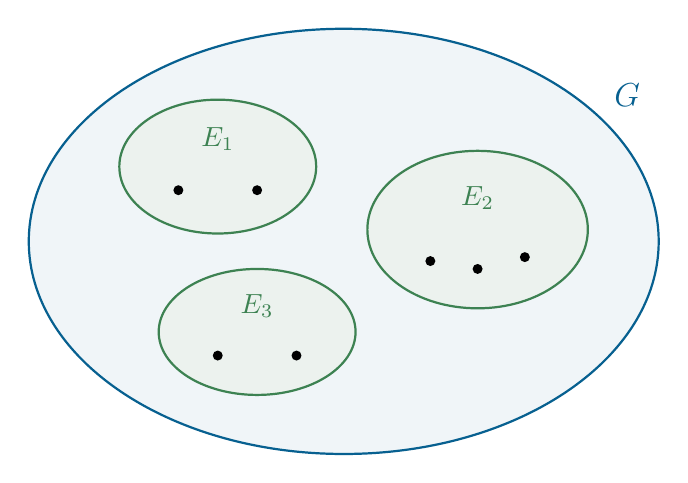
\begin{tikzpicture}
    % (1) Fill of G
    \fill[figBlue!6] (0, 0) ellipse (4.0 and 2.7);

    % (2) Fills of equivalence classes E_1, E_2, E_3
    \fill[figGreen!10] (-1.6, 0.95) ellipse (1.25 and 0.85);
    \fill[figGreen!10] (1.7, 0.15) ellipse (1.40 and 1.00);
    \fill[figGreen!10] (-1.1, -1.15) ellipse (1.25 and 0.80);

    % (3) Outlines
    \draw[thick, figBlue] (0, 0) ellipse (4.0 and 2.7);
    \draw[thick, figGreen] (-1.6, 0.95) ellipse (1.25 and 0.85);
    \draw[thick, figGreen] (1.7, 0.15) ellipse (1.40 and 1.00);
    \draw[thick, figGreen] (-1.1, -1.15) ellipse (1.25 and 0.80);

    % (4) Group elements as dots inside each class
    \fill (-2.1, 0.65) circle (1.8pt) (-1.1, 0.65) circle (1.8pt);
    \fill (1.1, -0.25) circle (1.8pt) (1.7, -0.35) circle (1.8pt) (2.3, -0.20) circle (1.8pt);
    \fill (-1.6, -1.45) circle (1.8pt) (-0.6, -1.45) circle (1.8pt);

    % (5) Text last
    \node[figGreen] at (-1.6, 1.30) {$E_1$};
    \node[figGreen] at (1.7, 0.55) {$E_2$};
    \node[figGreen] at (-1.1, -0.82) {$E_3$};
    \node[anchor=south west, inner sep=0.15cm, figBlue, font=\large] at (3.28, 1.55) {$G$};
\end{tikzpicture}
\end{center}

Summing the cardinalities of these disjoint classes accounts for every element of $G$ exactly once:
\begin{equation}\label{eq:lagrange-sum-classes}
|G| = \sum_{i=1}^k |E_i|,
\end{equation}
where $k$ is the number of equivalence classes.
\end{content}

\begin{speech}[00:20:32 - 00:22:30]
Okay. So, this fellow, Joseph-Louis, he was actually born Italian. And his name at birth was Giuseppe Luigi, as far as I can tell. But he became French somehow in his life. Yeah. His name was always Lagrange as far... but he was born in Turin \inlinemetanote{erases the lower-left and middle boards}. But then the standard place in the undergraduate curriculum where you learn the calculus of variations would be a mathematical class on classical mechanics, which is often taught probably in the physics department, I don't know. But that's probably the work that is his greatest work --- Lagrange's greatest work. This is not his greatest work. But it's very well known.

All right, so, what are we going to do here? We have to prove this, and the observation --- which is an incredibly simple observation --- so the claim, which will prove everything, is that for all equivalence classes, the size of this equivalence class is actually the size of $H$ \inlinemetanote{writes and boxes: Claim: $\forall i,\ |E_i| = |H|$}. All right? So, that sum is actually just adding up $H$, the order of $H$. And so, of course, that proves it.

So, claim: if I prove this --- so I have to prove this claim --- then Lagrange's theorem follows \inlinemetanote{writes: Then Lagrange's Thm follows:}. Then we rewrite that equation as: the size of $G$ is equal to the sum $i = 1$ to the $k$, $|E_i|$, but all of these are just the size of $H$, so this is actually $k$ times $|H|$ \inlinemetanote{writes: $|G| = \sum_{i=1}^k |E_i| = k \cdot |H|$}. So, that shows that... as a consequence, the order of $H$ divides the order of $G$ \inlinemetanote{writes: $\implies |H| \mid |G|\;\square$}. So, that's the end of the theorem, and I have just to prove this \inlinemetanote{points at the boxed claim}, okay?
\end{speech}

\begin{content}[Reduction of Lagrange's Theorem to Equal Class Sizes]
\begin{highlight}{MidnightBlue}[Key Claim]
\begin{claim}\label[claim]{clm:class-size-equals-h}
For all $i \in \{1, \dots, k\}$,
\[
|E_i| = |H|.
\]
\end{claim}
\end{highlight}

Assuming \cref{clm:class-size-equals-h}, Lagrange's theorem (\cref{thm:lagrange}) follows immediately from \eqref{eq:lagrange-sum-classes}:
\[
|G| = \sum_{i=1}^k |E_i| = \sum_{i=1}^k |H| = k \cdot |H| \implies |H| \mid |G|.
\]
It therefore remains only to prove \cref{clm:class-size-equals-h}.
\end{content}

\begin{aiNote}[Beyond the Lecture: The Index of a Subgroup]
% [PERSISTENT, ADDITION]
The integer $k = |G|/|H|$, counting the number of distinct equivalence classes (left cosets) of $H$ in $G$, is called the \newterm{index} of $H$ in $G$, conventionally denoted $[G : H] := k$. In particular, any subgroup of index $[G : H] = 2$ is automatically normal (proved in Week~9, \cref{prop:index-2-normal}).
\end{aiNote}

\subsection{Bijection Between \texorpdfstring{$H$}{H} and Each Equivalence Class}

\begin{speech}[00:22:30 - 00:23:52]
So, let us see: how are we going to prove that? So, let $E = E_i$ be an equivalence class in $G$ \inlinemetanote{writes: Let $E = E_i$ be an equiv. class in $G$}. So, we have some equivalence class in $G$: here is the picture of $G$, here is $E$ \inlinemetanote{writes $E \subset G$ and draws a region $G$ containing a smaller region $E$ with dots}. And I need to show that the cardinality of $E$ is exactly $|H|$.

So, the first thing I do is I reach into $E$ and I pick a person in it, which of course I call $x$ \inlinemetanote{marks a dot in $E$}, right? So, I have $x \in E$ \inlinemetanote{writes: $x \in E$}. I can do that because it's an equivalence class; it's not empty. We don't consider the empty equivalence class.

Okay, so, then I would like to make a map from $H$ to $E$ \inlinemetanote{writes: $\phi \colon H \to E$}, and I define this: $\phi(h)$ equals... \inlinemetanote{writes: $\phi(h) =$} and what do you think I'm going to write here? I have to write something that's definitely in $E$, and all I know about $E$ is it has $x$ in it, so you have to remember what this equivalence relation is. So, yeah, what would you propose I write? I can't... yeah?
\end{speech}

\begin{student}[Student Answer]
$xh$.
\end{student}

\begin{speech}[00:23:54 - 00:24:43]
$xh$ \inlinemetanote{writes: $xh$}. I have to write something, and whatever I write has to be in $E$. And the things that are in $E$, remember: $x$ is equivalent to $y$, that's if and only if we have this equation $xh = y$ for some $h$ in $H$ \inlinemetanote{writes: $x \sim y \iff xh = y, \text{ some } h \in H$}. So, these things for sure are equivalent to $x$. Is that clear? This is more or less the only thing you could possibly write in this situation.

So, that gives a map, so at least $\phi$ maps $H$ to $E$ \inlinemetanote{writes: At least $\phi \colon H \to E$}. That means if you put in any $h$ in here, you get something in the equivalence class.
\end{speech}

\begin{content}[Constructing the Map \texorpdfstring{$\phi \colon H \to E$}{phi: H -> E}]
Let $E = E_i \subset G$ be an arbitrary equivalence class in $G$. Since equivalence classes are non-empty, we may choose an element $x \in E$.

\definecolor{figBlue}{HTML}{076090} % RGB (7, 96, 144): petrol blue (MidnightBlue)
\definecolor{figGreen}{HTML}{3D8252} % RGB (61, 130, 82): dark green (ForestGreen!70!black)
\definecolor{figRed}{HTML}{B5261C} % RGB (181, 38, 28): brick red (BrickRed)
\begin{hidden}
- Canvas: no scale, cm; G = ellipse centre (0, 0), radii 3.2 and 2.1; E = ellipse centre (-0.2, -0.1), radii 1.65 and 1.15;
  picture x in [-3.2, 3.6], y in [-2.1, 2.1]
- Order: (1) fill of G (figBlue!6); (2) fill of E (figGreen!10); (3) outlines of G and E; (4) dots in E, x in figRed;
  (5) all text last
- Containment: E spans x in [-1.85, 1.45], y in [-1.25, 1.05]; farthest corner (-1.37, 0.71):
  (-1.37/3.2)^2 + (0.71/2.1)^2 = 0.18 + 0.11 = 0.29 < 1, well inside G.
- Dots in E: x = (-0.55, 0.10), other elements at (0.55, 0.20) and (0.20, -0.60).
- Labels (inner sep 0.15cm):
  "x" anchor south at x = (-0.55, 0.10): x in [-0.65, -0.45], y in [0.25, 0.70], 0.35 below E's top (1.05)
  "E" anchor south west at E's outline point (-0.2 + 1.65 cos 40, -0.1 + 1.15 sin 40) = (1.06, 0.64):
    x in [1.21, 1.41], y in [0.79, 1.24]; check corner (1.41, 1.24) in G: (1.41/3.2)^2 + (1.24/2.1)^2 = 0.19 + 0.35 = 0.54 < 1
  "G" anchor south west at G's outline point (3.2 cos 35, 2.1 sin 35) = (2.62, 1.20), outside G
\end{hidden}
\begin{center}
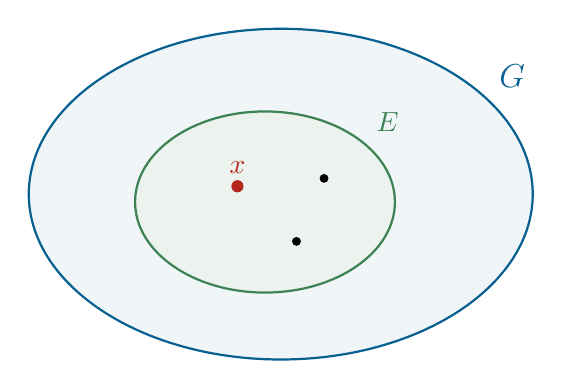
\begin{tikzpicture}
    % (1), (2) Fills
    \fill[figBlue!6] (0, 0) ellipse (3.2 and 2.1);
    \fill[figGreen!10] (-0.2, -0.1) ellipse (1.65 and 1.15);

    % (3) Outlines
    \draw[thick, figBlue] (0, 0) ellipse (3.2 and 2.1);
    \draw[thick, figGreen] (-0.2, -0.1) ellipse (1.65 and 1.15);

    % (4) Elements inside E
    \fill (0.55, 0.20) circle (1.6pt) (0.20, -0.60) circle (1.6pt);
    \fill[figRed] (-0.55, 0.10) circle (2.2pt);

    % (5) Text last
    \node[anchor=south, inner sep=0.15cm, figRed] at (-0.55, 0.10) {$x$};
    \node[anchor=south west, inner sep=0.15cm, figGreen] at (1.06, 0.64) {$E$};
    \node[anchor=south west, inner sep=0.15cm, figBlue, font=\large] at (2.62, 1.20) {$G$};
\end{tikzpicture}
\end{center}

We define a map $\phi \colon H \to E$ by:
\[
\phi(h) := xh.
\]
\textbf{Well-definedness (at least $\phi \colon H \to E$):} Recall that for any $y \in G$, $x \sim y \iff xh' = y$ for some $h' \in H$. For every $h \in H$, setting $y = xh$ gives $x \sim xh$. Since $x \in E$, every element equivalent to $x$ belongs to $E$, so $\phi(h) = xh \in E$ for all $h \in H$.
\end{content}

\begin{hidden}
% timestamp: 00:24:43
% topic: Proof of Lagrange's Theorem: map phi: H -> E defined
% board_state: thm:lagrange, clm:class-size-equals-h, eq:lagrange-sum-classes
% next_goal: Prove phi is a bijection (surjective and injective), concluding Lagrange's theorem.
% open_loops: none
\end{hidden}

\begin{speech}[00:24:43 - 00:26:58]
So, now we want to prove... the last step is we should prove, we will prove (let's be confident here) that $\phi$ is a bijection \inlinemetanote{writes: We will prove that $\phi$ is a bijection.}. So, if we do that, then we're happy because we need to show that the cardinality of $E$ is the same as the cardinality of $H$, and if I show this map is a bijection, then I will have shown that.

All right, so, for this, to start, we need to prove that $\phi$ is surjective \inlinemetanote{writes: $\bullet\ \phi$ is surjective}. And this is true because anybody in $E$ is someone that's related to $x$, and all people related to $x$ are of this form \inlinemetanote{points at $\phi(h) = xh$}. So, it's surjective by definition of this equivalence relation \inlinemetanote{writes: (True by def.)}. Meaning the only way to be in this equivalence class of $x$ is to satisfy such a relation for some $h$.

Okay, then we have to prove $\phi$ is injective, and then we will be done \inlinemetanote{writes: $\bullet\ \phi$ is injective.}. Okay, so, we have to prove this. Why? Why would this be true? So, injectivity means we have to study the equation $\phi(h_1) = \phi(h_2)$ \inlinemetanote{writes: $\phi(h_1) = \phi(h_2), \ h_1, h_2 \in H$}. We have to study that equation, right?

So, let's see: suppose $\phi(h_1) = \phi(h_2)$ where $h_1$ and $h_2$ are in $H$. So, we suppose this is true. Well, what do we do next? We write down the definitions: this thing is $x h_1$, and that should equal $x h_2$ \inlinemetanote{writes: $G \ni x h_1 = x h_2$}. All right. But this is an equation that holds in the group. So, well, now we use the cancellation property, so by the cancellation property, we can get rid of this \inlinemetanote{cancels $x$ on both sides}. So, this implies $h_1 = h_2$, and that's injectivity \inlinemetanote{writes: $\implies h_1 = h_2\;\square$}. So, we finished the proof.
\end{speech}

\begin{content}[Proof of Bijectivity and Unified Proof of Lagrange's Theorem]
\begin{proof}[Proof of \cref{clm:class-size-equals-h}]
We show that $\phi \colon H \to E$, $\phi(h) = xh$, is a bijection.

\textbf{Surjectivity:} Let $y \in E$ be arbitrary. Because $E$ is the equivalence class containing $x$, we have $x \sim y$. By the definition \eqref{eq:coset-equiv-relation} of $\sim$, there exists $h \in H$ such that $xh = y$, i.e., $\phi(h) = y$. Hence, $\phi$ is surjective (directly by definition).

\textbf{Injectivity:} Suppose $\phi(h_1) = \phi(h_2)$ for $h_1, h_2 \in H$. By definition of $\phi$, this means:
\[
x h_1 = x h_2.
\]
Using the left cancellation property in the group $G$ (\cref{prop:cancellation-laws}, equivalently multiplying both sides on the left by $x^{-1}$), we cancel $x$:
\[
\cancel{x} h_1 = \cancel{x} h_2 \implies h_1 = h_2.
\]
Hence, $\phi$ is injective.

Since $\phi \colon H \to E$ is both surjective and injective, it is a bijection, so $|E| = |H|$.
\end{proof}

\begin{steps}[Complete Summary of the Proof of Lagrange's Theorem]
Combining all steps gives the complete proof of \cref{thm:lagrange}:
\begin{enumerate}[label=\textbf{\arabic*.}]
    \item Define $x \sim y \stackrel{\text{def}}{\iff} \exists h \in H \text{ such that } xh = y$. The subgroup axioms of $H$ guarantee that $\sim$ is reflexive ($e \in H$), symmetric ($h^{-1} \in H$), and transitive ($h_1 h_2 \in H$).
    \item Because $G$ is finite, $\sim$ partitions $G$ into finitely many disjoint equivalence classes $E_1, \dots, E_k$, so $|G| = \sum_{i=1}^k |E_i|$.
    \item For each $i \in \{1, \dots, k\}$, choosing $x \in E_i$, the map $\phi \colon H \to E_i$ given by $\phi(h) = xh$ is a bijection (surjective by definition of $\sim$, injective by group cancellation), so $|E_i| = |H|$ for every $i$.
    \item Therefore, $|G| = k \cdot |H|$, which proves $|H| \mid |G|$.
\end{enumerate}
\end{steps}
\end{content}
\end{proofWrapper}

\begin{speech}[00:26:58 - 00:27:49]
Yeah, that's the whole proof. It's an extremely simple proof, and if you understand it, you will never forget it.

So, when you first see this, it's a very strange property that if you have these groups, these finite groups, and you assemble these subgroups, you can try as hard as you want, but you'll never be able to make a subgroup that doesn't have order which divides the group. In particular, if your group has prime order, it's extremely hard to make subgroups, because there's very few numbers that divide prime numbers. So, this is going to be used over and over again in the study of finite groups \inlinemetanote{erases the lower board}.
\end{speech}

\begin{content}
\begin{remark}[Subgroups of Groups of Prime Order]\label[remark]{rem:prime-order-groups}
By Lagrange's theorem (\cref{thm:lagrange}), if a finite group $G$ has prime order $|G| = p$, the only possible orders for a subgroup $H \subset G$ are $1$ and $p$. Consequently, any group of prime order has no proper non-trivial subgroups (only $\{e\}$ and $G$ itself). In particular, choosing any $x \in G \setminus \{e\}$ yields a subgroup $\langle x \rangle \subset G$ with $1 < |\langle x \rangle|$ and $|\langle x \rangle| \mid p$, forcing $|\langle x \rangle| = p = |G|$, so $\langle x \rangle = G$ and $\operatorname{Ord}(x) = p$; by \cref{cor:cyclic-subgroup-isomorphism}, every group of prime order $p$ is cyclic ($G \cong \bigl(\faktor{\mathbb{Z}}{p\mathbb{Z}}, +, 0\bigr)$; revisited in Week~9, \cref{clm:prime-order-cyclic}).
\end{remark}
\end{content}

\section{Examples of Groups}

\subsection{Cycle Decomposition in the Symmetric Group \texorpdfstring{$S_n$}{Sn}}

\begin{speech}[00:27:49 - 00:29:43]
Okay, I wanted to do some examples of groups, because that's the fun part of group theory --- or at least for me, the fun part of group theory is this rich source of examples \inlinemetanote{erases the lower-left and middle boards}.

So, I mean, I can't somehow say enough how much you should understand, how much you should make sure you understand $S_n$, understand the cycle notation, etc. It's extremely important: if you learn anything in this class that you'll learn later in your life, you'll regret not thinking about $S_n$.

So, let me say some more comments about it. Maybe I say it again just because I don't know whether you've... but this is actually --- I don't know whether this is all things you've studied before or not --- but $S_n$ I write now \inlinemetanote{writes $S_n$ and draws a region with six dots}: this is not $S_n$, this is the set of $n$ points, so I should maybe write it differently \inlinemetanote{erases the region with dots}. I'll try to say one more thing about the cycle notation, because as I said, it's extremely important, and it's not like I gave you a totally formal presentation of the cycle notation. I gave you a little bit and it's kind of your responsibility to work out the cycle notation from that, but I'll give you one more hint.

So, if I take here the set $[n]$, which is the set $1, 2, 3$... and now I write them as dots, $n$ \inlinemetanote{writes: $[n] = \{ \bullet, \bullet, \bullet, \dots, \bullet \}$ with numbers underneath}. Okay, let's make it $7$. Is that $7$? Four, five, six, seven, very good \inlinemetanote{labels the seven dots $1, 2, 3, 4, 5, 6, 7$}.

Okay, so, this is my set; if I take an element in here, in $S_7$, then it maps this set... it's a bijection \inlinemetanote{changes $S_n$ to $S_7 \ni \sigma$ and writes \qt{$\sigma \colon [n] \to [n]$}}. That's by definition: it's a bijection from this set to itself.
\end{speech}

\begin{content}[{Permutations as Bijections on \texorpdfstring{$[n]$}{[n]}}]
\begin{notation}[{The Set \texorpdfstring{$[n]$}{[n]} and Symmetric Group \texorpdfstring{$S_7$}{S7}}]\label[notation]{not:set-n-bijection}
We denote the finite set of $n$ elements by $[n] := \{1, 2, \dots, n\}$ (taking $n = 7$ as a concrete example, $[7] = \{1, 2, 3, 4, 5, 6, 7\}$). An element $\sigma \in S_n$ (here $\sigma \in S_7$, \cref{def:symmetric-group}) is, by definition, a bijection:
\[
\sigma \colon [n] \to [n].
\]
\end{notation}
\end{content}

\begin{speech}[00:29:43 - 00:31:21]
So, how do I see the cycles, if I want to see it as a picture? So, I pick $1$, and $\sigma$ takes it to somewhere, so maybe $\sigma$ takes $1$ to $4$ \inlinemetanote{draws an arrow from $1$ to $4$ labeled $\sigma$}. It has to go somewhere, and then maybe it goes to $6$ \inlinemetanote{draws an arrow from $4$ to $6$}. It keeps going, but eventually this path has to repeat, right? Because there's only finitely many elements; it can't keep going to different points, eventually it has to repeat.

Could it repeat like this \inlinemetanote{draws a tentative arrow from $6$ back to $4$}? Could it be like going here, here, here, here? And the answer is no, because it's a bijection. We already know who comes to that \inlinemetanote{points at $4$}; there can't be something else that comes to that. So, it cannot repeat like that \inlinemetanote{erases the arrow from $6$ to $4$}. It has to repeat, and the only way it can repeat is to go back to the beginning \inlinemetanote{draws an arrow from $6$ back to $1$ underneath}. That's the only way it can repeat.

So, another way to think about these cycles is just you look at it dynamically: there's the seven points, or however many points; you pick $1$, it goes, and eventually it comes back to $1$, and that's the cycle for $1$. And in this case, it would be $(1\,4\,6)$ \inlinemetanote{writes: $(1\,4\,6)$}.

And then we take this stuff out and we go with the points that are remaining, again. Now we start with $2$: $2$ has to go, and has to be a cycle, and has to come back to $2$, and it can never interfere with the cycle here because of the bijective property. So, you just take out another cycle. You do that, and now you get the cycle decomposition. So, let's pretend here $2$ goes to $3$ and comes back, then this would be $(2\,3)$ \inlinemetanote{draws arrows between $2$ and $3$ and writes: $(2\,3)$}. And what's left? $7$ by himself \inlinemetanote{draws a loop at $7$ and writes: $(7)$}, all right? So, that would be in this case, but that's how you visually see it.
\end{speech}

\begin{content}[Visualizing Cycle Decomposition (Initial Sketch)]
Following the action of a bijection $\sigma \in S_7$ dynamically on the elements $\{1, 2, 3, 4, 5, 6, 7\}$ must eventually repeat because the set is finite. Because $\sigma$ is injective, no two elements can map to the same target; thus, the path starting at $1$ cannot branch into an already-visited interior point (such as $4$), and the only way it can repeat is by returning directly to its starting point $1$. Removing that cycle and repeating on the remaining elements produces disjoint cycles.

\definecolor{figBlue}{HTML}{076090} % RGB (7, 96, 144): petrol blue (MidnightBlue)
\definecolor{figGreen}{HTML}{3D8252} % RGB (61, 130, 82): dark green (ForestGreen!70!black)
\definecolor{figOrange}{HTML}{CC7E2B} % RGB (204, 126, 43): ochre orange (BurntOrange!80!black)
\begin{hidden}
- Canvas: no scale, cm; seven circular nodes v1..v7 (radius 0.28cm, minimum size 0.56cm) at y = 0,
  x = 1.5, 3.3, 5.1, 6.9, 8.7, 10.5, 12.3 (spacing 1.8cm). Picture spans x in [1.2, 13.5], y in [-1.4, 1.9].
- Order: (1) vertices v1..v7; (2) arrows for cycle (1 4 6) in figBlue, (2 3) in figGreen, self-loop at v7 in figOrange;
  (3) label \sigma last
- Arrows:
  v1 -> v4 above: (v1.north) .. controls (2.5, 1.9) and (5.9, 1.9) .. (v4.north); apex y = 0.25*0.28 + 0.75*1.9 = 1.50
  v4 -> v6 above: (v4.60) .. controls (7.8, 1.85) and (9.6, 1.85) .. (v6.120); apex y ~ 1.46
  v6 -> v1 below: (v6.south) .. controls (9.5, -1.6) and (2.5, -1.6) .. (v1.south); nadir y = -1.27
  v2 -> v3 above: (v2.north) .. controls (3.8, 0.75) and (4.6, 0.75) .. (v3.north); apex y = 0.63 (below 1->4 which is > 1.2 at x=3.3..5.1)
  v3 -> v2 below: (v3.south) .. controls (4.6, -0.75) and (3.8, -0.75) .. (v2.south); nadir y = -0.63 (above 6->1 which is < -1.1 at x=3.3..5.1)
  v7 self-loop: \path (v7) edge[loop right, min distance=8mm] (v7);
- Note: 5 is momentarily omitted on the board before the lecturer notices and corrects it in the next step.
- Label "\sigma" anchor south at (4.2, 1.55), inner sep 0.15cm, above the apex (4.2, 1.50) of v1 -> v4.
\end{hidden}
\begin{center}
\begin{tikzpicture}[>=Stealth]
    % (1) Vertices 1..7
    \node[circle, draw, minimum size=0.56cm, inner sep=0pt] (v1) at (1.5, 0) {$1$};
    \node[circle, draw, minimum size=0.56cm, inner sep=0pt] (v2) at (3.3, 0) {$2$};
    \node[circle, draw, minimum size=0.56cm, inner sep=0pt] (v3) at (5.1, 0) {$3$};
    \node[circle, draw, minimum size=0.56cm, inner sep=0pt] (v4) at (6.9, 0) {$4$};
    \node[circle, draw, minimum size=0.56cm, inner sep=0pt] (v5) at (8.7, 0) {$5$};
    \node[circle, draw, minimum size=0.56cm, inner sep=0pt] (v6) at (10.5, 0) {$6$};
    \node[circle, draw, minimum size=0.56cm, inner sep=0pt] (v7) at (12.3, 0) {$7$};

    % (2) Cycle (1 4 6), Cycle (2 3), and initial loop on 7 (5 temporarily missed)
    \draw[->, thick, figBlue] (v1.north) .. controls (2.5, 1.9) and (5.9, 1.9) .. (v4.north);
    \draw[->, thick, figBlue] (v4.60) .. controls (7.8, 1.85) and (9.6, 1.85) .. (v6.120);
    \draw[->, thick, figBlue] (v6.south) .. controls (9.5, -1.6) and (2.5, -1.6) .. (v1.south);
    \draw[->, thick, figGreen] (v2.north) .. controls (3.8, 0.75) and (4.6, 0.75) .. (v3.north);
    \draw[->, thick, figGreen] (v3.south) .. controls (4.6, -0.75) and (3.8, -0.75) .. (v2.south);
    \path[->, thick, figOrange] (v7) edge[loop right, min distance=8mm] (v7);

    % (3) Text last
    \node[anchor=south, inner sep=0.15cm, figBlue] at (4.2, 1.55) {$\sigma$};
\end{tikzpicture}
\end{center}

Initial incomplete board expression (element $5$ momentarily omitted):
\[
(1\,4\,6)(2\,3)(7) \quad \text{(Incomplete)}
\]
\end{content}

\begin{hidden}
% timestamp: 00:31:21
% topic: Symmetric group S_7 cycle decomposition initial sketch
% board_state: not:set-n-bijection
% next_goal: Correct omitted element 5 to (5 7), relate cycle lengths to partitions, introduce Platonic solids.
% open_loops: none
\end{hidden}

\begin{speech}[00:31:21 - 00:32:34]
You notice: out of this cycle decomposition --- and this would be for $\sigma$ \inlinemetanote{writes \qt{$\sigma =$} to the left of $(1\,4\,6)(2\,3)(7)$} --- you get a certain set of numbers: the lengths of the cycles. And you get $7$ equals... \inlinemetanote{writes: $7 =$} I don't know, it's not working. We missed one! $5$, sorry \inlinemetanote{draws arrows between $5$ and $7$ and changes $(7)$ to $(5\,7)$}. There. You get $7$ is equal to $3 + 2 + 2$ \inlinemetanote{writes: $3 + 2 + 2$}.

So, whenever you have... because at the end you have to account for all the points --- every point has to be in one of the cycles --- so you get all the points and that's the lengths of the cycles. So, this gives you a connection to partitions, and that's an extremely deep connection. So, this is a partition, do you know that? That's like an object, how to take a number and break it up into other numbers. So, there's a very deep connection between the symmetric group and the study of partitions \inlinemetanote{writes: $S_n \longleftrightarrow \operatorname{Part}(n)$}.

Maybe I'll say a little bit about this later, but have you ever thought about this, the study of partitions? Maybe I'll say a little bit about it. But not today. That's a great subject --- okay, but not today.
\end{speech}

\begin{content}[Correction: Including Element 5 and Connection to Partitions]
Recognizing that element $5$ had been omitted from the initial diagram, the lecturer links $5$ and $7$ into a $2$-cycle $(5\,7)$, giving the complete disjoint cycle decomposition:
\[
\sigma = (1\,4\,6)(2\,3)(5\,7).
\]

\definecolor{figBlue}{HTML}{076090} % RGB (7, 96, 144): petrol blue (MidnightBlue)
\definecolor{figGreen}{HTML}{3D8252} % RGB (61, 130, 82): dark green (ForestGreen!70!black)
\definecolor{figOrange}{HTML}{CC7E2B} % RGB (204, 126, 43): ochre orange (BurntOrange!80!black)
\begin{hidden}
- Canvas: no scale, cm; same seven nodes v1..v7 at x = 1.5, 3.3, 5.1, 6.9, 8.7, 10.5, 12.3, y = 0. Picture x in [1.2, 12.6], y in [-1.4, 1.9].
- Order: (1) vertices v1..v7; (2) arrows for (1 4 6) in figBlue, (2 3) in figGreen, and corrected (5 7) in figOrange;
  (3) label \sigma last
- Corrected cycle (5 7):
  v5 -> v7 above: (v5.north) .. controls (9.6, 0.95) and (11.4, 0.95) .. (v7.north); apex y = 0.25*0.28 + 0.75*0.95 = 0.78;
    crosses v4->v6 cleanly near x = 9.9 (where v4->v6 descends from 1.46 to 0.28) in a distinct hue (figOrange vs figBlue)
  v7 -> v5 below: (v7.south) .. controls (11.4, -0.85) and (9.6, -0.85) .. (v5.south); nadir y = -0.71 (above v6->v1 which is at -1.07 around x=8.7, crossing cleanly near x = 9.95)
- Label "\sigma" anchor south at (4.2, 1.55), inner sep 0.15cm.
\end{hidden}
\begin{center}
\begin{tikzpicture}[>=Stealth]
    % (1) Vertices 1..7
    \node[circle, draw, minimum size=0.56cm, inner sep=0pt] (v1) at (1.5, 0) {$1$};
    \node[circle, draw, minimum size=0.56cm, inner sep=0pt] (v2) at (3.3, 0) {$2$};
    \node[circle, draw, minimum size=0.56cm, inner sep=0pt] (v3) at (5.1, 0) {$3$};
    \node[circle, draw, minimum size=0.56cm, inner sep=0pt] (v4) at (6.9, 0) {$4$};
    \node[circle, draw, minimum size=0.56cm, inner sep=0pt] (v5) at (8.7, 0) {$5$};
    \node[circle, draw, minimum size=0.56cm, inner sep=0pt] (v6) at (10.5, 0) {$6$};
    \node[circle, draw, minimum size=0.56cm, inner sep=0pt] (v7) at (12.3, 0) {$7$};

    % (2) Disjoint cycles (1 4 6), (2 3), and (5 7)
    \draw[->, thick, figBlue] (v1.north) .. controls (2.5, 1.9) and (5.9, 1.9) .. (v4.north);
    \draw[->, thick, figBlue] (v4.60) .. controls (7.8, 1.85) and (9.6, 1.85) .. (v6.120);
    \draw[->, thick, figBlue] (v6.south) .. controls (9.5, -1.6) and (2.5, -1.6) .. (v1.south);
    \draw[->, thick, figGreen] (v2.north) .. controls (3.8, 0.75) and (4.6, 0.75) .. (v3.north);
    \draw[->, thick, figGreen] (v3.south) .. controls (4.6, -0.75) and (3.8, -0.75) .. (v2.south);
    \draw[->, thick, figOrange] (v5.north) .. controls (9.6, 0.95) and (11.4, 0.95) .. (v7.north);
    \draw[->, thick, figOrange] (v7.south) .. controls (11.4, -0.85) and (9.6, -0.85) .. (v5.south);

    % (3) Text last
    \node[anchor=south, inner sep=0.15cm, figBlue] at (4.2, 1.55) {$\sigma$};
\end{tikzpicture}
\end{center}

Because every element of $[7]$ belongs to a unique cycle in the disjoint cycle decomposition, the cycle lengths sum to $7$:
\[
7 = 3 + 2 + 2.
\]
% [BOARD-CHECKED: frame 00:32:30 (2026-11-18): the board has S_n <-> Part(n), with 7 = 3 + 2 + 2 below it]
This decomposition yields an integer \newterm{partition} of $n$, a way to break $n$ up into a sum of positive integers, where the order of the summands does not matter. Writing $\operatorname{Part}(n)$ for the set of partitions of $n$, this gives a deep connection:
\[
S_n \longleftrightarrow \operatorname{Part}(n).
\]
Week~8 makes it exact: the conjugacy classes of $S_n$ correspond bijectively to the partitions of $n$ (\cref{thm:sn-conjugacy-classes-partitions}, \cref{cor:conjugacy-classes-partitions}), and their number is the partition function $p(n)$ (\cref{def:partition-function}, \cref{thm:euler-partition-product}).
\end{content}

\subsection{Rotational Symmetry Groups of the Platonic Solids}

\begin{speech}[00:32:34 - 00:33:22]
So, I want to do some examples. And the example should be symmetry groups of geometric objects, and the most famous geometric objects are the Platonic solids --- in some sense, the most famous.

You could take the tetrahedron \inlinemetanote{draws a tetrahedron}, the cube \inlinemetanote{draws a cube}, and then there's the octahedron --- I'm not gifted \inlinemetanote{draws an octahedron}, but that's not terrible --- and then there's a dodecahedron, which is much harder to draw \inlinemetanote{draws a dodecahedron}, you know, I don't know, but you know what this thing is, right? But that's not bad, so this is the one with $12$ sides \inlinemetanote{writes \qt{$12$} underneath the dodecahedron}. And then of course there's the icosahedron, which is even more complicated to draw \inlinemetanote{draws an icosahedron}.

So, those are the five Platonic solids...
\end{speech}

\begin{content}[The Five Platonic Solids]
The five Platonic solids --- the regular, convex polyhedra in $\mathbb{R}^3$ whose faces are congruent regular polygons and whose vertices have identical valency --- provide classic geometric examples of finite symmetry groups:

\definecolor{figBlue}{HTML}{076090} % RGB (7, 96, 144): petrol blue (MidnightBlue)
\definecolor{figGray}{HTML}{666665} % RGB (102, 102, 101): dark gray (gray!80!black)
\begin{hidden}
- Canvas: no scale, cm; five polyhedra arranged horizontally, centres at x = 1.2, 3.9, 6.6, 9.3, 12.0 (2.7 cm apart),
  vertical range y in [0.03, 1.87], captions below at y = -0.25. Picture spans x in [0.0, 13.2], y in [-1.2, 1.9].
- Order: (1) dashed hidden edges (where drawn); (2) solid visible edges; (3) text captions last
- Coordinates (each solid ~1.8 wide, gap ~0.9 between neighbouring solids):
  1. Tetrahedron (x around 1.2): T=(1.2, 1.85), L=(0.4, 0.40), F=(1.3, 0.15), R=(2.0, 0.55); hidden L--R dashed.
  2. Cube (x around 3.9): front (3.1, 0.25)-(4.2, 1.35), back shifted +(0.5, 0.45) to (3.6, 0.70)-(4.7, 1.80);
     hidden edges meeting at back-bottom-left (3.6, 0.70) dashed.
  3. Octahedron (x around 6.6): N=(6.6, 1.85), S=(6.6, 0.05), W=(5.8, 0.95), F=(6.45, 0.70), E=(7.4, 0.95), B=(6.75, 1.20);
     back edges meeting at B dashed.
  4. Dodecahedron (x around 9.3, centre C4=(9.3, 0.95), orthographic front projection looking down a 5-fold face axis):
     outer decagon r_2 = 0.92 at 90, 126, 162, 198, 234, 270, 306, 342, 18, 54 deg;
     inner front pentagon r_1 = r_2 / phi = 0.92 / 1.618 = 0.57 at 90, 162, 234, 306, 18 deg;
     5 radial spokes from (a:0.57) to (a:0.92), forming 1 central regular pentagon + 5 surrounding pentagons.
  5. Icosahedron (x around 12.0, centre C5=(12.0, 0.95)): inner triangle r=0.44 at 90, 210, 330 deg;
     outer hexagon r=0.90 at 30, 90, 150, 210, 270, 330 deg; each inner vertex a connects to outer a and a+-60.
- Captions: anchor north at (x_i, -0.25), text width 2.3cm, align flush center, 0.4 apart;
  under Dodecahedron: "Dodecahedron\\($12$ faces)" preserving the board's "12".
\end{hidden}
\begin{center}
\begin{tikzpicture}[thick]
    % 1. Tetrahedron
    \draw[dashed, figGray] (0.4, 0.40) -- (2.0, 0.55);
    \draw[figBlue] (1.2, 1.85) -- (0.4, 0.40) -- (1.3, 0.15) -- (2.0, 0.55) -- (1.2, 1.85) -- (1.3, 0.15);

    % 2. Cube
    \draw[dashed, figGray] (3.1, 0.25) -- (3.6, 0.70) -- (4.7, 0.70) (3.6, 0.70) -- (3.6, 1.80);
    \draw[figBlue] (3.1, 0.25) rectangle (4.2, 1.35);
    \draw[figBlue] (3.1, 1.35) -- (3.6, 1.80) -- (4.7, 1.80) -- (4.2, 1.35);
    \draw[figBlue] (4.2, 0.25) -- (4.7, 0.70) -- (4.7, 1.80);

    % 3. Octahedron
    \draw[dashed, figGray] (6.6, 1.85) -- (6.75, 1.20) -- (6.6, 0.05) (5.8, 0.95) -- (6.75, 1.20) -- (7.4, 0.95);
    \draw[figBlue] (6.6, 1.85) -- (5.8, 0.95) -- (6.6, 0.05) -- (7.4, 0.95) -- (6.6, 1.85) -- (6.45, 0.70) -- (6.6, 0.05);
    \draw[figBlue] (5.8, 0.95) -- (6.45, 0.70) -- (7.4, 0.95);

    % 4. Dodecahedron (front orthographic projection)
    \coordinate (C4) at (9.3, 0.95);
    \draw[figBlue] ($(C4)+(90:0.57)$) -- ($(C4)+(162:0.57)$) -- ($(C4)+(234:0.57)$)
        -- ($(C4)+(306:0.57)$) -- ($(C4)+(18:0.57)$) -- cycle;
    \draw[figBlue] ($(C4)+(90:0.92)$) -- ($(C4)+(126:0.92)$) -- ($(C4)+(162:0.92)$)
        -- ($(C4)+(198:0.92)$) -- ($(C4)+(234:0.92)$) -- ($(C4)+(270:0.92)$)
        -- ($(C4)+(306:0.92)$) -- ($(C4)+(342:0.92)$) -- ($(C4)+(18:0.92)$)
        -- ($(C4)+(54:0.92)$) -- cycle;
    \foreach \a in {90, 162, 234, 306, 18} {
        \draw[figBlue] ($(C4)+(\a:0.57)$) -- ($(C4)+(\a:0.92)$);
    }

    % 5. Icosahedron (front projection)
    \coordinate (C5) at (12.0, 0.95);
    \draw[figBlue] ($(C5)+(90:0.44)$) -- ($(C5)+(210:0.44)$) -- ($(C5)+(330:0.44)$) -- cycle;
    \draw[figBlue] ($(C5)+(30:0.90)$) -- ($(C5)+(90:0.90)$) -- ($(C5)+(150:0.90)$) -- ($(C5)+(210:0.90)$)
        -- ($(C5)+(270:0.90)$) -- ($(C5)+(330:0.90)$) -- cycle;
    \foreach \a [evaluate=\a as \am using \a-60, evaluate=\a as \ap using \a+60] in {90, 210, 330} {
        \draw[figBlue] ($(C5)+(\a:0.44)$) -- ($(C5)+(\a:0.90)$);
        \draw[figBlue] ($(C5)+(\a:0.44)$) -- ($(C5)+(\am:0.90)$);
        \draw[figBlue] ($(C5)+(\a:0.44)$) -- ($(C5)+(\ap:0.90)$);
    }

    % Text last
    \node[anchor=north, text width=2.3cm, align=flush center, font=\small] at (1.2, -0.25) {Tetrahedron};
    \node[anchor=north, text width=2.3cm, align=flush center, font=\small] at (3.9, -0.25) {Cube};
    \node[anchor=north, text width=2.3cm, align=flush center, font=\small] at (6.6, -0.25) {Octahedron};
    \node[anchor=north, text width=2.3cm, align=flush center, font=\small] at (9.3, -0.25) {Dodecahedron\\($12$ faces)};
    \node[anchor=north, text width=2.3cm, align=flush center, font=\small] at (12.0, -0.25) {Icosahedron};
\end{tikzpicture}
\end{center}
\end{content}

\begin{speech}[00:33:22 - 00:35:30]
...and one thing in this class, at some point, you should be familiar with what the groups of rotational symmetries of these objects are. And if you remember a long time ago --- well, it couldn't be that long, since the beginning of the class --- we discussed this. So, for every one of these there's a group of rotational symmetries, which means you imagine this object and you look at the rotations that move the faces to the faces. And we discussed this one before. So, this one \inlinemetanote{points at the cube}, let's just review this: how many rotational symmetries does this have \inlinemetanote{writes under the cube: how many rotations?}?

So, you just imagine you have a cube, and you can just... really you could just pick up a cube and do this: how many ways can you rotate it? And the group is rotation and composition. The neutral element is \qt{do nothing}. And the inverse element is \qt{undo what you did}. That's the proof it's a group. So, how many rotational symmetries does this have? You can just like rotate the cube in your head.

The standard way to count this --- there's many different ways to count it --- but one way to count it is you take the top side. You can suppose, just take like the top of the box. You can ask: how many ways can I rotate it in keeping that the top of the box? And the answer is clearly four; you can, you know, rotate it this... I mean, if you want to keep it to be the top, there's four things you can do. Do you agree? So, that's four \inlinemetanote{writes: $4$}.

And what else can you do? I can move the top of the box to any other side. And how many sides are there? Six. And it turns out that's all you can do, because you can just think about it. I've already... I mean, yeah, you should think about this yourself. That's the only thing you can do: you can either rotate the box or move it to that side \inlinemetanote{writes: $4 \cdot 6 = 24$}.

But these things, I said, this is the geometric part of the class, and geometry is all about the camera in your head, and at some point, if you want to understand geometry, you have to develop the camera in your head; there's no other way, in some sense. Okay, and I can't really help you do that.
\end{speech}

\begin{content}[Rotational Symmetries of the Cube]
For any Platonic solid, the set of rotational symmetries forms a group under composition:
\begin{itemize}
    \item \textbf{Operation:} Composition of $3\text{D}$ rotations carrying the solid onto itself (faces to faces).
    \item \textbf{Neutral element:} Doing nothing (the identity rotation).
    \item \textbf{Inverse:} Undoing a rotation (rotating by the opposite angle about the same axis).
\end{itemize}

\begin{example}[Counting the Rotational Symmetries of a Cube]\label[example]{ex:cube-rotations-count}
To count the number of rotations of a cube:
\begin{itemize}
    \item Fixing which face sits on top, there are $4$ rotations that keep that face on top (rotations by $0^\circ, 90^\circ, 180^\circ, 270^\circ$).
    \item The top face can be moved to any of the $6$ faces of the cube.
\end{itemize}
Therefore, the total number of rotational symmetries is:
\[
4 \cdot 6 = 24.
\]
\end{example}
\end{content}

\begin{speech}[00:35:30 - 00:35:45]
So, what about this one \inlinemetanote{points at the tetrahedron}? How many rotational symmetries does this have? So, this time you should use the same logic.
\end{speech}

\begin{student}[Student Answer]
Twelve.
\end{student}

\begin{speech}[00:35:47 - 00:35:50]
Twelve, twelve is good. Why do you say it's twelve?
\end{speech}

\begin{student}[Student Answer, continued]
If I fix the lower... the bottom...
\end{student}

\begin{speech}[00:35:53 - 00:35:54]
Yeah.
\end{speech}

\begin{student}[Student Answer, continued]
...I can rotate it \inlinemetanote{partially inaudible}...
\end{student}

\begin{speech}[00:35:55 - 00:35:56]
Three ways, exactly.
\end{speech}

\begin{student}[Student Answer, continued]
...and then \inlinemetanote{partially inaudible} by four.
\end{student}

\begin{speech}[00:35:58 - 00:36:06]
Yeah, so, this and this way --- there's lots of different ways, there's no unique way to do it. This one is, well, I don't know, $3 \times 4 = 12$ \inlinemetanote{writes under the tetrahedron: $3 \cdot 4 = 12$}.
\end{speech}

\begin{content}[Rotational Symmetries of the Tetrahedron]
\begin{example}[Counting the Rotational Symmetries of a Tetrahedron]\label[example]{ex:tetrahedron-rotations-count}
Fixing one triangular face at the bottom, there are $3$ rotations keeping it at the bottom, and that face can be moved to any of the $4$ faces of the tetrahedron:
\[
3 \cdot 4 = 12.
\]
\end{example}
\end{content}

\begin{speech}[00:36:06 - 00:36:39]
And what about this one \inlinemetanote{points at the octahedron}? So, let's just do this together: we could pick one of the triangles --- do you know what these things are, right? You've seen them? It's not, you know... So, if you take one of the triangle sides, there's three motions around, and eight ways it can go, so it's $24$ also. We'll leave these \inlinemetanote{points at the dodecahedron and icosahedron}; these are more fun and we'll discuss them later. These are easy to think about, relatively.
\end{speech}

\begin{content}[Rotational Symmetries of the Octahedron]
\begin{example}[Counting the Rotational Symmetries of an Octahedron]\label[example]{ex:octahedron-rotations-count}
Fixing one triangular face, there are $3$ rotational symmetries that preserve that face, and $8$ triangular faces to which it can be sent:
\[
3 \cdot 8 = 24.
\]
\end{example}

\begin{steps}[Why the Face-Counting Rule Applies to Platonic Solids]
Unlike an arbitrary polyhedron, a Platonic solid has congruent regular polygonal faces on which its rotational symmetry group $\operatorname{Rot}(P)$ acts transitively: any chosen face can be rotated onto any other face, and the rotations keeping a face in place are the in-plane rotations of that regular polygon. Thus, for all five Platonic solids,
\[
|\operatorname{Rot}(P)| = (\text{rotations keeping one face in place}) \times (\text{number of faces}),
\]
which likewise gives $5 \cdot 12 = 60$ for the dodecahedron and $3 \cdot 20 = 60$ for the icosahedron (deferred to Week~9, \cref{thm:platonic-solids-symmetries}; this face-counting paradigm is formalized via the Orbit--Stabilizer Theorem, \cref{thm:orbit-stabilizer}).
\end{steps}
\end{content}

\begin{hidden}
% timestamp: 00:36:39
% topic: Platonic solids rotational symmetry counts (cube: 24, tetrahedron: 12, octahedron: 24)
% board_state: ex:cube-rotations-count, ex:tetrahedron-rotations-count, ex:octahedron-rotations-count
% next_goal: Ask whether Rot(cube) is isomorphic to S_4 and prove it geometrically via the 4 long diagonals.
% open_loops: dodecahedron and icosahedron symmetry groups deferred to later lecture
\end{hidden}

\subsection{Isomorphism Between the Rotation Group of the Cube and \texorpdfstring{$S_4$}{S4}}

\begin{speech}[00:36:39 - 00:38:42]
This one \inlinemetanote{points at the cube} is a super fun thing to think about. So, that's a group of order $24$. So, the rotations of this cube is a group of order $24$ \inlinemetanote{writes \qt{$\operatorname{Rot}(\square)$ is grp. of order $24$}, a small cube drawn inside the parentheses}. What group is it? Do you know any groups of order $24$?

Well, $24$ happens to be a factorial. $24$ happens to be $4$ factorial. That's a group of order $24$ factorial (i.e., $24$). But we know another group of order $24$: $S_4$ is also a group of order $24$ \inlinemetanote{writes: $S_4$}. So, this is now a beautiful geometric question: is this rotational group, this rotations here --- I guess this cube, this is bad terminology, but anyway, it's not great notation, but it's very convincing if I do it --- is it isomorphic to $S_4$ \inlinemetanote{writes \qt{Is $\operatorname{Rot}(\square)$} and \qt{$\cong S_4$?}}? That's a beautiful question, and I don't know whether I should solve it for you or not... Like, maybe I solve it for you --- I do this one for you.

There's, again, many ways you can do this. One way to do it is you write down the multiplication table for this rotation group: you name all $24$ elements --- you have to make up your own names, now you can be like Fred, Bob, Jane, you can just name whatever you want --- you name $24$ elements here, you name the $24$ elements for the $S_4$, and those are already named by the cycle decompositions, and then you find some bijection that respects the product. That is a hard way to do it, but you could do it that way. It's a hard way to do it because you have two sets of $24$ elements and very few of them are the correct bijection. So, that's not a great way of doing it.

There is a beautiful way of doing it which I will show you in a moment, and it's kind of... maybe it's good to show this because it shows, you know, the power of geometry here.
\end{speech}

\begin{content}[Identifying the Rotation Group of the Cube]
The group of rotational symmetries $\operatorname{Rot}(\text{Cube})$ is a finite group of order $24 = 4!$, matching the order $|S_4| = 4! = 24$ of the symmetric group $S_4$.

\begin{question}\label[question]{q:rot-cube-s4}
Is the rotation group of the cube isomorphic to $S_4$, i.e.,
\[
\operatorname{Rot}(\text{Cube}) \cong S_4?
\]
\end{question}
\end{content}

\begin{aiNote}[Pictogram Notation and Spoken Slip (\texorpdfstring{$24!$ vs.\ $24$}{24! vs. 24})]
% [PERSISTENT]
On the blackboard, the lecturer draws a small wireframe cube inside $\operatorname{Rot}(\dots)$ instead of writing the word \qt{cube}; we denote this $\operatorname{Rot}(\text{Cube})$. In the audio, the lecturer also briefly misspeaks \qt{$24$ factorial} when referring to the order $24 = 4!$ of $\operatorname{Rot}(\text{Cube})$ and $S_4$.
\end{aiNote}

\begin{speech}[00:38:42 - 00:40:54]
So, it helps here to have a professor who's artistically gifted, and you do not have this luck, unfortunately \inlinemetanote{draws a cube on the lower-middle board}. This is not a hard diagram; I should be able to handle it. So, here is the cube, all right?

And it turns out there is a set of four things here --- there's a beautiful geometric set of four things --- and those are the four long diagonals. So, if I take this point of the cube, there's an opposite point, and there's a long diagonal \inlinemetanote{draws the first long diagonal across the cube}. Okay? So, if you imagine a box, for every point in the cube there's an opposite point. Meaning if that point has coordinates $+1, +1, +1$ in the cube, it's $-1, -1, -1$, if the cube has side length $2$ --- so, it has an opposite, and there's one of them. And there's eight vertices, so there's four long diagonals.

So, I'll try to draw them; I don't know if it's so helpful... \inlinemetanote{draws two more long diagonals passing through the center} Ah, it's not so good --- they all pass through the origin \inlinemetanote{marks the center in red chalk}. I think I missed one, too: one, two... where is it? One, two, three... this one. No, this one's hidden, yeah, it's there \inlinemetanote{draws the fourth long diagonal}. Okay. I told you. So, there's one, two, three, four.

But still, I said, it's much better to have the camera in your head: there's the box, and there's four long diagonals; they all go through the middle, this origin. Is that clear?

And now, they shouldn't all be... you label these, let's say $a, b, c, d$ --- which is, where is $d$? $d$ \inlinemetanote{labels the four long diagonals $a$, $b$, $c$, $d$}. So, there's four of them; you give them different names. And you can see now when you rotate this cube, you permute these four long diagonals. That's just a fact; I mean, you move them, the long diagonals go to other long diagonals. So, that's kind of an amazing thing; that shows that there is a way to get... a rotation of the cube gives you a permutation of the long diagonals.
\end{speech}

\begin{content}[The Four Long Diagonals of the Cube]
A cube $[-1, 1]^3$ of side length $2$ centered at the origin has $8$ vertices $(\pm 1, \pm 1, \pm 1)$, arranged in $4$ pairs of opposite vertices $\pm v$. Connecting each opposite pair produces $4$ \newterm{long diagonals} $a, b, c, d$, all passing through the origin:

\definecolor{figBlue}{HTML}{076090} % RGB (7, 96, 144): petrol blue (MidnightBlue)
\definecolor{figGreen}{HTML}{3D8252} % RGB (61, 130, 82): dark green (ForestGreen!70!black)
\definecolor{figOrange}{HTML}{CC7E2B} % RGB (204, 126, 43): ochre orange (BurntOrange!80!black)
\definecolor{figRed}{HTML}{B5261C} % RGB (181, 38, 28): brick red (BrickRed)
\definecolor{figGray}{HTML}{666665} % RGB (102, 102, 101): dark gray (gray!80!black)
\definecolor{figLightGray}{HTML}{A6A6A5} % RGB (166, 166, 165): light gray (gray!70)
\begin{hidden}
- Canvas: no scale, cm; parallel 3D projection x = (1, 0), y = (13/18, 6/18), z = (0, 1) with half-side s = 1.8,
  so a point (x, y, z) lands at (x + (13/18) y, z + (6/18) y); half-depth shift is (1.3, 0.6), full front-to-back shift is (2.6, 1.2).
  Picture spans x in [-3.6, 3.6], y in [-2.5, 3.1].
- 8 cube vertices (exact page coordinates):
  Vppp = ( 1.8,  1.8,  1.8) = ( 3.1,  2.4)   Vpmp = ( 1.8, -1.8,  1.8) = ( 0.5,  1.2)
  Vmpp = (-1.8,  1.8,  1.8) = (-0.5,  2.4)   Vmmp = (-1.8, -1.8,  1.8) = (-3.1,  1.2)
  Vppm = ( 1.8,  1.8, -1.8) = ( 3.1, -1.2)   Vpmm = ( 1.8, -1.8, -1.8) = ( 0.5, -2.4)
  Vmpm = (-1.8,  1.8, -1.8) = (-0.5, -1.2)   Vmmm = (-1.8, -1.8, -1.8) = (-3.1, -2.4)
- Order: (1) hidden cube edges meeting at Vmpm (-0.5, -1.2), dashed figLightGray; (2) visible cube edges, figGray;
  (3) four long diagonals through (0, 0): a (Vmmp--Vppm, figBlue), b (Vmpp--Vpmm, figGreen), c (Vppp--Vmmm, figOrange),
  d (Vpmp--Vmpm, figRed); (4) centre origin dot in figRed; (5) labels a, b, c, d last
- Labels (normal size, 0.20 per character, height 0.45, inner sep 0.15cm):
  "a" anchor east at Vmmp = (-3.1, 1.2): x in [-3.45, -3.25], y in [0.98, 1.42]; nothing left of -3.1.
  "b" anchor south at Vmpp = (-0.5, 2.4): x in [-0.60, -0.40], y in [2.55, 3.00]; nothing above 2.4.
  "c" anchor south west at Vppp = (3.1, 2.4): x in [3.25, 3.45], y in [2.55, 3.00]; nothing right/above (3.1, 2.4).
  "d" anchor south east at Vpmp = (0.5, 1.2): x in [0.15, 0.35], y in [1.35, 1.80].
- Collisions check for "d":
  front-top edge (y = 1.2) is 0.15 below; top-right depth edge starts at (0.5, 1.2), 0.21 from (0.35, 1.35);
  back-top edge (y = 2.4) is 0.60 above; diagonal b passes y = 1.35 at x = -0.28, 0.43 to the left;
  diagonal d ends at (0.5, 1.2), 0.21 away. All four labels are >= 0.15cm clear of every edge and diagonal.
\end{hidden}
\begin{center}
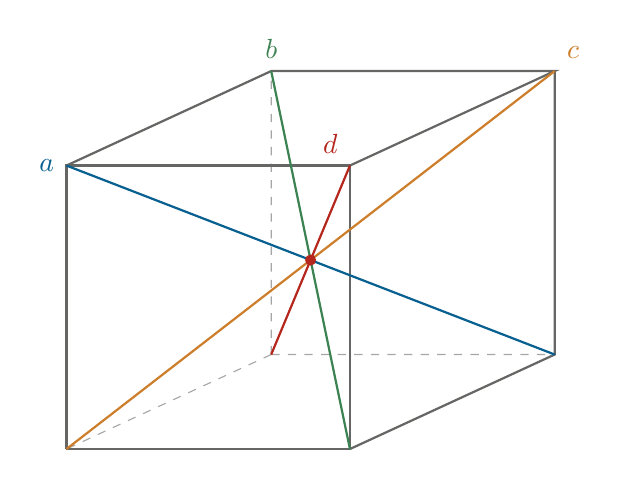
\begin{tikzpicture}
    % Coordinates
    \coordinate (Vppp) at (3.1, 2.4);
    \coordinate (Vpmp) at (0.5, 1.2);
    \coordinate (Vmpp) at (-0.5, 2.4);
    \coordinate (Vmmp) at (-3.1, 1.2);
    \coordinate (Vppm) at (3.1, -1.2);
    \coordinate (Vpmm) at (0.5, -2.4);
    \coordinate (Vmpm) at (-0.5, -1.2);
    \coordinate (Vmmm) at (-3.1, -2.4);

    % (1) Hidden edges meeting at back-bottom-left Vmpm
    \draw[dashed, figLightGray] (Vmpm) -- (Vmpp) (Vmpm) -- (Vppm) (Vmpm) -- (Vmmm);

    % (2) Visible edges of the cube
    \draw[thick, figGray] (Vmmm) -- (Vpmm) -- (Vpmp) -- (Vmmp) -- (Vmmm);
    \draw[thick, figGray] (Vmmp) -- (Vmpp) -- (Vppp) -- (Vpmp);
    \draw[thick, figGray] (Vpmm) -- (Vppm) -- (Vppp);

    % (3) The four long diagonals passing through the origin (0, 0)
    \draw[thick, figBlue] (Vmmp) -- (Vppm);
    \draw[thick, figGreen] (Vmpp) -- (Vpmm);
    \draw[thick, figOrange] (Vppp) -- (Vmmm);
    \draw[thick, figRed] (Vpmp) -- (Vmpm);

    % (4) Origin dot
    \fill[figRed] (0, 0) circle (2pt);

    % (5) Text last
    \node[anchor=east, inner sep=0.15cm, figBlue] at (Vmmp) {$a$};
    \node[anchor=south, inner sep=0.15cm, figGreen] at (Vmpp) {$b$};
    \node[anchor=south west, inner sep=0.15cm, figOrange] at (Vppp) {$c$};
    \node[anchor=south east, inner sep=0.15cm, figRed] at (Vpmp) {$d$};
\end{tikzpicture}
\end{center}

Any rotation of the cube must carry opposite vertices to opposite vertices, and therefore permutes the four long diagonals $\{a, b, c, d\}$.
\end{content}

\begin{speech}[00:40:54 - 00:42:34]
And the proof is just that: take the rotations of this cube --- this is a group --- and there's a homomorphism to the permutation group of the long diagonals, which is $S_4$ \inlinemetanote{writes: $\operatorname{Rot}(\square) \xrightarrow{\phi} S_4$}. And the claim is this: rotations go to permutations of the long diagonals \inlinemetanote{writes: $\phi \colon$ rotations $\to$ permutations of the long diagonals}. I say long diagonals all the time here, but I mean, you know, if you pick two points on the same face, then there's kind of a short diagonal that's on the side, but there's four... so, every time you rotate, you permute the long diagonals. And the claim is this is an isomorphism \inlinemetanote{writes: This is an iso.}.

So, how are you going to prove this is an isomorphism? It's not going to be too hard: you just have to check every time you rotate, you do move some long diagonal --- it's not trivial. Because the groups already have order $24$, so if it's injective, then it has to be surjective. Or you could also prove it's injective and surjective. But you have to think about how, when you move this cube, it cannot be the case that if you do a non-trivial rotation, all the long diagonals stay fixed.

So, I leave that to you to think about. But that's a totally geometric proof, a beautiful geometric proof, which is way better than trying to write down this table, which, you know, probably you will not succeed in doing.
\end{speech}

\begin{content}[Isomorphism \texorpdfstring{$\operatorname{Rot}(\text{Cube}) \cong S_4$}{Rot(Cube) isomorphic to S4}]
\begin{answer}[to \cref{q:rot-cube-s4}]\label[answer]{ans:rot-cube-s4}
\textcolor{ForestGreen}{\textbf{Yes}}, $\operatorname{Rot}(\text{Cube}) \cong S_4$.
\end{answer}

\begin{theorem}[Rotational Symmetry Group of the Cube]\label[theorem]{thm:cube-rotations-isomorphism}
The group of rotational symmetries of a cube is isomorphic to the symmetric group on four letters:
\[
\operatorname{Rot}(\text{Cube}) \cong S_4.
\]
\end{theorem}

Consider the group homomorphism
\[
\phi \colon \operatorname{Rot}(\text{Cube}) \to S_4, \qquad \text{Rotation} \mapsto \text{permutation of the long diagonals } \{a, b, c, d\}.
\]
Since $|\operatorname{Rot}(\text{Cube})| = 24 = |S_4|$, proving that $\phi$ is injective automatically implies that $\phi$ is bijective, and hence an isomorphism (this is left to the reader).

\begin{proof}[Proof of Injectivity (beyond the lecture)]
The lecture leaves injectivity to the students (\qt{I leave that to you to think about}). Let the four long diagonals of $[-1, 1]^3$ be spanned by the vectors
\[
v_1 = (1, 1, 1), \quad v_2 = (-1, 1, 1), \quad v_3 = (1, -1, 1), \quad v_4 = (1, 1, -1).
\]
Suppose a rotation $R \in \operatorname{Rot}(\text{Cube})$ lies in $\ker(\phi)$, meaning $R$ maps each long diagonal line $\mathbb{R}v_i$ onto itself. Since $R$ preserves lengths and sends vertices to vertices, we must have $R v_i = \lambda_i v_i$ with $\lambda_i \in \{+1, -1\}$ for each $i \in \{1, 2, 3, 4\}$.

Observe that $v_1 = v_2 + v_3 + v_4$, and that $\{v_2, v_3, v_4\}$ is linearly independent in $\mathbb{R}^3$ (its determinant is $4 \neq 0$). By linearity of $R$:
\[
\lambda_1 (v_2 + v_3 + v_4) = \lambda_1 v_1 = R(v_1) = R(v_2) + R(v_3) + R(v_4) = \lambda_2 v_2 + \lambda_3 v_3 + \lambda_4 v_4.
\]
Comparing coefficients in the basis $\{v_2, v_3, v_4\}$ forces $\lambda_1 = \lambda_2 = \lambda_3 = \lambda_4$. If all four were $-1$, then $R = -I$, which has determinant $\det(-I) = (-1)^3 = -1$, contradicting the fact that every rotation has $\det(R) = +1$. Thus, $\lambda_1 = \lambda_2 = \lambda_3 = \lambda_4 = +1$, so $R$ fixes a basis of $\mathbb{R}^3$ and hence, $R = I$. Therefore, $\ker(\phi)$ is trivial, $\phi$ is injective, and by equal finite cardinalities $|\operatorname{Rot}(\text{Cube})| = |S_4| = 24$, $\phi$ is an isomorphism.
\end{proof}
\end{content}

\begin{hidden}
% timestamp: 00:42:34
% topic: Proof that Rot(cube) \cong S_4 via permutation of the 4 long diagonals
% board_state: q:rot-cube-s4, ans:rot-cube-s4, thm:cube-rotations-isomorphism
% next_goal: Study Rot(tetrahedron) -> S_4 (image A_4) and why Rot(cube) -> S_8 is not an isomorphism.
% open_loops: none
\end{hidden}

\subsection{Rotational Symmetries of the Tetrahedron and the Cube's Vertices}

\begin{speech}[00:42:34 - 00:43:31]
Okay, so, we have one more moment here. So, what about this one \inlinemetanote{draws a tetrahedron on the lower-left board}? This is order $12$, right? We said that the rotations of this has order $12$ \inlinemetanote{writes: $\operatorname{Rot}(\triangle)$ and \qt{$\text{ord} = 12$} beneath it}. This sits inside... there's a homomorphism here to $S_4$ again, because any rotation permutes the four vertices \inlinemetanote{writes \qt{$\xrightarrow{\tilde{\phi}} S_4$} and \qt{$24$} beneath $S_4$}.

It's a different geometric object: here \inlinemetanote{points at the cube}, this is a much more sophisticated thing, the long diagonals; this one's kind of obvious: every time I rotate, I permute the four vertices. And this is also injective. But this is not an isomorphism: this is $24$, this is order $12$; it goes to a subgroup, and that subgroup's a very well-known, important subgroup --- it's called $A_4$. So, the answer... I'm not defining this now, but this is just the name: this thing here is actually isomorphic to what's called $A_4$; we'll talk about it more \inlinemetanote{writes: $A_4 \cong \operatorname{Rot}(\triangle)$}. So, it's not the whole thing.
\end{speech}

\begin{content}[Homomorphism from \texorpdfstring{$\operatorname{Rot}(\text{Tetrahedron})$}{Rot(Tetrahedron)} to \texorpdfstring{$S_4$}{S4}]
\definecolor{figBlue}{HTML}{076090} % RGB (7, 96, 144): petrol blue (MidnightBlue)
\definecolor{figGray}{HTML}{666665} % RGB (102, 102, 101): dark gray (gray!80!black)
\begin{hidden}
- Canvas: no scale, cm; tetrahedron vertices: P1=(0, 2.4), P2=(-1.5, -0.3), P3=(0.3, -0.8), P4=(1.7, 0.2).
  Picture spans x in [-2.0, 2.2], y in [-1.4, 2.9].
- Order: (1) hidden back edge P2--P4 dashed figGray; (2) solid front edges; (3) vertex dots in figBlue;
  (4) vertex labels 1, 2, 3, 4 (augmented to match the homomorphism into S_4) last
- Labels (inner sep 0.15cm):
  "1" anchor south at P1 (0, 2.4); "2" anchor north east at P2 (-1.5, -0.3);
  "3" anchor north at P3 (0.3, -0.8); "4" anchor west at P4 (1.7, 0.2).
  All four labels sit outside the tetrahedron silhouette in wide free angles.
\end{hidden}
\begin{center}
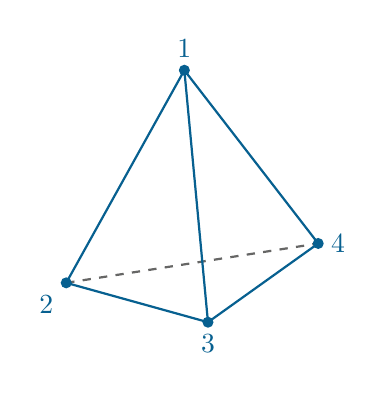
\begin{tikzpicture}[thick]
    \coordinate (P1) at (0, 2.4);
    \coordinate (P2) at (-1.5, -0.3);
    \coordinate (P3) at (0.3, -0.8);
    \coordinate (P4) at (1.7, 0.2);

    % (1) Back edge dashed
    \draw[dashed, figGray] (P2) -- (P4);

    % (2) Visible edges
    \draw[figBlue] (P1) -- (P2) -- (P3) -- (P4) -- (P1) -- (P3);

    % (3) Vertices
    \fill[figBlue] (P1) circle (2pt) (P2) circle (2pt) (P3) circle (2pt) (P4) circle (2pt);

    % (4) Text last (augmented vertex labels illustrating the permutation action)
    \node[anchor=south, inner sep=0.15cm, figBlue] at (P1) {$1$};
    \node[anchor=north east, inner sep=0.15cm, figBlue] at (P2) {$2$};
    \node[anchor=north, inner sep=0.15cm, figBlue] at (P3) {$3$};
    \node[anchor=west, inner sep=0.15cm, figBlue] at (P4) {$4$};
\end{tikzpicture}
\end{center}

\begin{theorem}[Rotational Symmetry Group of the Tetrahedron]\label[theorem]{thm:tetrahedron-isomorphism}
The group of rotational symmetries of a regular tetrahedron is isomorphic to a subgroup $A_4$ of $S_4$:
\[
\operatorname{Rot}(\text{Tetrahedron}) \cong A_4.
\]
\end{theorem}

For the tetrahedron, there is an analogous group homomorphism induced by permuting the $4$ vertices:
\[
\operatorname{Rot}(\text{Tetrahedron}) \xrightarrow{\tilde{\phi}} S_4,
\]
where $|\operatorname{Rot}(\text{Tetrahedron})| = 12$ and $|S_4| = 24$. While $\tilde{\phi}$ is injective, it cannot be surjective (and hence is not an isomorphism) because $12 < 24$. Instead, its image is a subgroup of order $12$ inside $S_4$ called $A_4$ (to be defined in the next week, \cref{def:alternating-group}, \cref{thm:rot-tetrahedron-a4}):
\[
A_4 \cong \operatorname{Rot}(\text{Tetrahedron}).
\]
\end{content}

\begin{aiNote}[Beyond the Lecture: The Alternating Group \texorpdfstring{$A_4$}{A4}]
% [PERSISTENT, ADDITION]
The subgroup $A_4 \subset S_4$ is the \newterm{alternating group} of degree $4$, consisting of all even permutations of four elements (of order $4! / 2 = 12$; see \cref{def:alternating-group} and \cref{thm:rot-tetrahedron-a4}). Injectivity of $\tilde{\phi} \colon \operatorname{Rot}(\text{Tetrahedron}) \to S_4$ holds because any rotation fixing all $4$ vertices of the regular tetrahedron fixes three linearly independent vectors in $\mathbb{R}^3$ (e.g., from the centroid to three vertices) and hence must be the identity. Geometrically, the $12$ rotations of the regular tetrahedron correspond to the identity, eight $3$-cycles ($\pm 120^\circ$ rotations around a vertex and the center of the opposite face), and three products of two disjoint $2$-cycles such as $(1\,2)(3\,4)$ ($180^\circ$ rotations around midpoints of opposite edges): $1 + 8 + 3 = 12$.
\end{aiNote}

\begin{speech}[00:43:31 - 00:43:54]
You could say: why didn't we do that here \inlinemetanote{points at the cube}? The rotation group also has a homomorphism to the permutation group of the eight vertices. It does, but that's clearly not an isomorphism because $8$ factorial is a lot bigger than $24$ factorial (i.e., $24$). Okay, so, I stop.
\end{speech}

\begin{aiNote}[Spoken Slip and Vertex Action on the Cube]
% [PERSISTENT]
At the end of the lecture, the lecturer again says \qt{$24$ factorial} when referring to the order $24$ of $\operatorname{Rot}(\text{Cube})$, contrasting it with $|S_8| = 8!$, the size of the permutation group of the $8$ vertices of the cube. Because $|S_8| = 8! > 24$, the homomorphism $\operatorname{Rot}(\text{Cube}) \to S_8$ cannot be an isomorphism onto $S_8$.
\end{aiNote}

\begin{aiNote}[Beyond the Lecture: Injectivity of the Vertex Action on the Cube]
% [PERSISTENT, ADDITION]
Permuting the $8$ vertices gives a homomorphism $\operatorname{Rot}(\text{Cube}) \to S_8$. It is injective because a rotation fixing all $8$ vertices fixes $\mathbb{R}^3$ and is the identity. Its image is a subgroup of order $24$, tiny inside $S_8$, since $|S_8| = 8! = 40\,320 \gg 24$.
\end{aiNote}

\begin{overview}[Summary of Key Concepts]
\begin{itemize}
    \item \textbf{Finite and Non-Abelian Perspective:} Group theory here focuses primarily on finite and not necessarily Abelian groups, bracketed by the rich family of symmetric groups $S_n$ ($|S_n| = n!$) and the cyclic Abelian groups $(\faktor{\mathbb{Z}}{n\mathbb{Z}}, +, 0)$.
    \item \textbf{Element Order and Generated Subgroup:} For $x \in G$ in a finite group $G$, $\operatorname{Ord}(x) := \min \{ m \in \mathbb{Z}_{>0} \mid x^m = e \}$ is well-defined, and the set $\langle x \rangle := \{e, x, x^2, \dots, x^{\operatorname{Ord}(x)-1}\} \subset G$ is a subgroup (the subgroup generated by $x$) isomorphic to $(\faktor{\mathbb{Z}}{\operatorname{Ord}(x)\mathbb{Z}}, +, 0)$.
    \item \textbf{Lagrange's Theorem:} For every finite group $G$ and subgroup $H \subset G$, $|H| \mid |G|$. The proof defines the equivalence relation $x \sim y \stackrel{\text{def}}{\iff} \exists h \in H \text{ such that } xh = y$ on $G$, partitions $G$ into equivalence classes $E_1, \dots, E_k$, and shows via $\phi \colon H \to E_i$, $\phi(h) = xh$, that $|E_i| = |H|$ for all $i$. As consequences, $\operatorname{Ord}(x) \mid |G|$ for every $x \in G$, and groups of prime order have no proper non-trivial subgroups.
    \item \textbf{Cycle Decomposition and Partitions:} Viewing a permutation $\sigma \in S_n$ as a bijection $[n] \to [n]$ decomposes $[n]$ into disjoint cycles whose lengths sum to $n$ (for instance, $\sigma = (1\,4\,6)(2\,3)(5\,7) \in S_7$ gives $7 = 3 + 2 + 2$), connecting $S_n$ to integer partitions.
    \item \textbf{Rotational Symmetries of Platonic Solids:} Under composition of rotations, $|\operatorname{Rot}(\text{Cube})| = 4 \cdot 6 = 24$, $|\operatorname{Rot}(\text{Tetrahedron})| = 3 \cdot 4 = 12$, and $|\operatorname{Rot}(\text{Octahedron})| = 3 \cdot 8 = 24$. Permuting the $4$ long diagonals of the cube defines a homomorphism $\operatorname{Rot}(\text{Cube}) \to S_4$ that is an isomorphism $\operatorname{Rot}(\text{Cube}) \cong S_4$ (with injectivity left to the reader), whereas permuting the $4$ vertices of the tetrahedron defines an injective homomorphism $\operatorname{Rot}(\text{Tetrahedron}) \to S_4$ with image $A_4 \cong \operatorname{Rot}(\text{Tetrahedron})$ of order $12$.
\end{itemize}
\end{overview}